
% !TeX spellcheck = pt_BR
% !TEX encoding = UTF-8 Unicode

\chapter{Fundamentos}
\label{Cap_Fundam}

\citacao{A good course is a course with many stupid 
questions.}{Wendelin Werner, medalhista Fields 2006}

\citacao{Quem faz uma pergunta boba 
fica com vergonha $5$ segundos. Quem não pergunta nada fica 
bobo para sempre...}{Um faxineiro do ICEx, 2008}

\ifdefined\updateans
% Only need to run once in a lifetime, when the file ans.tex needs to be updated.
\Writetofile{ans}{\protect\section*{Capítulo \ref{Cap_Fundam}}}
\fi

\emph{Cálculo} lida com funções de uma ou mais variáveis reais. 
Portanto, ele necessita de uma compreensão boa das principais propriedades dos 
números reais, e suas manipulações na resolução de problemas elementares.\\

Esse capítulo contém lembretes sobre a aritmética elementar dos números reais, 
assim como a descrição de certos conjuntos do plano cartesiano, como retas e
círculos.
\emph{Não pretendemos dar uma exposição completa sobre esses assuntos}, mas 
apenas lembrar alguns fatos e estabelecer notações a respeito de coisas
elementares conhecidas pelo leitor.\\

A matéria desse capítulo será usada constantemente no restante da apostila: é 
importante o leitor verificar que ele consegue fazer todos os exercícios.

\section{Números reais}\index{números! reais $\bR$}
O conjunto dos números reais, $\bR$, pode ser visto como o conjunto dos pontos 
da linha real, que serão em geral denotados por letras minúsculas: $x,y,s,t,u$,
etc.
$\bR$ é munido de quatro operações aritméticas básicas: \grasA{adição} ($+$), 
\grasA{subtração} ($-$), \grasA{multiplicação} ($\times$ ou 
$\cdot$) e \grasA{divisão} ($\div$, ou simplesmente $/$).\\

Lembremos a importância de dois números com papel relevante com respeito à 
adição e multiplicação. Primeiro, o elemento $0$ (``zero'') é tal que $x+0=0+x=x$,
$x\cdot 0=0\cdot x=0$ para todo $x$. 
Um real $x$ diferente de zero será às vezes chamado de \grasA{não-nulo}.\\

Por outro lado, o elemento $1$ (``um'') é tal que $x\cdot 1=1\cdot x=x$ 
para todo $x\in \bR$.
É importante lembrar que \emph{a divisão por zero não é definida}\index{divisão por zero}.
Portanto, 
símbolos do tipo $x/0$ ou $0/0$ não fazem sentido. No entanto, $0/x=0$ para todo
$x\neq 0$.\\

Os subconjuntos de $\bR$ serão em geral denotados usando letras maiúsculas.
Por exemplo, $A=\{0,1,2\}$ é o conjunto que contém os três números reais $0,1$ 
e $2$, e $B=(0,2)$ é o intervalo aberto que contém todos os reais entre $0$ e
$2$ (ver abaixo).
O conjunto dos \grasA{números naturais é}~\footnote{Ao longo da apostila,
o símbolo ``$\pardef$'' será usado para definir um objeto. Por exemplo,
$A\pardef\{x\in \bR: x^2>1\}$ significa que $A$ é \emph{definido} como o conjunto
dos números reais cujo quadrado é maior que $1$.}\index{números! naturais $\bN$}
$$\bN\pardef \{1,2,3,\dots\}\,,$$
e o conjunto dos \grasA{inteiros}\index{números! inteiros $\bZ$} é
$$\bZ\pardef \{\dots,-3,-2,-1,0,1,2,3,\dots\}\,.$$


As operações entre conjuntos são: \grasA{interseção} ($\cap$), \grasA{união} 
($\cup$), \grasA{diferença} ($\setminus$). 
O \grasA{conjunto vazio} será denotado por $\varnothing$.

\subsection{Equações do primeiro e segundo grau}\label{SecEquacoes}
\index{equação! do primeiro grau}
Considere a equação do primeiro grau: 
\eq{\label{eqsimples}
1+4x=-7\,.}
\emph{Resolver} essa equação
significa achar o(s) valor(es) da variável $x$ para os quais a igualdade em \eqref{eqsimples} 
é verdadeira. Esse conjunto de valores será denotado por $S$ e chamado \grasA{conjunto de
soluções}\index{equação! conjunto de soluções}. 
A resolução é bem conhecida:
isolando $x$ obtemos 
uma única solução $x=-2$. Portanto, o conjunto das soluções de \eqref{eqsimples} é $S=\{-2\}$.\\


Considere em seguida a equação do segundo grau\index{equação! do segundo grau}:
\eq{\label{eqsimples2}
x^2=9\,.}
Aqui, sabemos que existem duas soluções, $x=\pm \sqrt{9}=\pm 3$, logo $S=\{+3,-3\}$. \\

Agora, já que um número negativo não possui raiz quadrada, a equação
$$
x^2=-4
$$
não possui nenhuma solução real: $S=\varnothing$. Finalmente, 
$$x^2=0$$
possui uma única solução: $S=\{0\}$.\\

 Um outro jeito de entender \eqref{eqsimples2} é de escrevê-la $x^2-9=0$ e de fatorar o
polinômio $x^2-9$, obtendo um produto de dois fatores:
$$(x-3)(x+3)=0\,.$$
 Para o produto de dois fatores (aqui, $x-3$ e $x+3$) ser zero, é necessário que pelo
menos um deles seja nulo. Se for o primeiro, $x-3=0$, então $x=3$. Se for o segundo,
$x+3=0$, logo $x=-3$. 
De modo geral, para $x$ ser solução de uma equação da forma 
\eq{\label{eq0}(x-\alpha)(x-\beta)=0\,,}
pelo menos um dos fatores, $(x-\alpha)$ ou $(x-\beta)$, deve ser igual a zero, o que 
 implica $x=\alpha$ ou $x=\beta$. Portanto, o conjunto das soluções de \eqref{eq0} é dado
por 
$S=\{\alpha,\beta\}$.\\

Olhemos agora para a equação do segundo grau da forma geral
\eq{\label{eq1}ax^2+bx+c=0\,.}
Se $a=0$, essa equação é do primeiro grau,
$$bx+c=0\,,$$
e a sua única solução é dada por $x=-\frac{c}{b}$ (supondo $b\neq 0$). Isto é,
$S=\{-\frac{c}{b}\}$. Por outro lado, se $a\neq 0$, então dividindo \eqref{eq1} por $a$, e
\emph{completando o quadrado}\index{completar um quadrado} obtemos:
\begin{align*}
0= x^2+\tfrac{b}{a}x+\tfrac{c}{a}&=(x+\tfrac{b}{2a})^2-(\tfrac{b}{2a})^2+\tfrac{c}{a}\,.
\end{align*}
Portanto,
$$(x+\tfrac{b}{2a})^2=(\tfrac{b}{2a})^2-\tfrac{c}{a}=\tfrac{b^2-4ac}{4a^2}\,.$$
Defina $\Delta\pardef b^2-4ac$. Se $\Delta<0$, não tem soluções:
$S=\varnothing$.
Se $\Delta\geq 0$, podemos tomar a raiz quadrada\index{raiz! quadrada} em ambos lados
dessa última expressão, e obter 
$$x+\tfrac{b}{2a}=\pm\tfrac{\sqrt{\Delta}}{2a}\,.$$
Isto é,
\eq{x=\tfrac{-b\pm\sqrt{\Delta}}{2a}\,.}
Resumindo: quando $a\neq 0$, o conjunto das soluções de \eqref{eq1} é dado por
$$S=
\begin{cases}
 \varnothing&\text{ se }\Delta<0\,\text{(zero soluções)}\\
\{\tfrac{-b}{2a}\}&\text{ se }\Delta=0\,\text{(uma solução)}\\
\{\tfrac{-b\pm \sqrt{\Delta}}{2a}\}&\text{ se }\Delta>0\, \text{(duas soluções)}\,.
\end{cases}
$$
\begin{exo}
Resolva as seguintes equações.
\begin{multicols}{3}
\begin{enumerate}
 \item\label{it0} $1-x=1$
 \item\label{it01} $x^2=1$
\item \label{it02} $\frac{1}{x}=x+1$
 \item\label{it1} $(x+1)(x-7)=0$
 \item\label{it2} $x=x$
 \item\label{it20} $x=x^2$
 \item\label{it3} $1=0$
\item \label{it4} $6x^3-1=3x(1+2x^2)$
\item \label{it500} $(x+6)(x+1)=1$ 
\end{enumerate}
\end{multicols}
\vspace{0.01cm}
\begin{sol}
\eqref{it0} $S=\{0\}$ 
\eqref{it01} $S=\{\pm 1\}$ 
 \eqref{it02} Observe primeiro que $0$ não é solução (a divisão por zero no lado esquerdo
não é nem definida). Assim, multiplicando por $x$ e rearranjando obtemos $x^2+x-1=0$. Como
$\Delta=5>0$, obtemos duas soluções: $S=\{\tfrac{-1\pm \sqrt{5}}{2}\}$. (Obs: o número
$\tfrac{-1+\sqrt{5}}{2}=0.618033989...$ é às vezes chamado de \grasA{razão áurea}. Veja 
$\verb|http://pt.wikipedia.org/wiki/Proporção_áurea|$)
 \eqref{it1} Para ter $(x+1)(x-7)=0$, é necessário que pelo menos um dos fatores, $(x+1)$
ou $(x-7)$, seja nulo. Isto é, basta ter $x=-1$ ou $x=7$. Assim, $S=\{-1,7\}$. Obs:
querendo aplicar a fórmula $x=\frac{-b\pm\sqrt{b^2-4ac}}{2a}$ de qualquer jeito, um aluno
com pressa pode querer expandir o produto $(x+1)(x-7)$ para ter $x^2-6x-7=0$, calcular
$\Delta=(-6)^2-4\cdot 1\cdot (-7)=64$, e obter 
$S=\{\frac{-(-6)\pm\sqrt{64}}{2\cdot 1}\}=\{-1,7\}$.
 Mas além de mostrar uma falta de compreensão (pra que expandir uma expressão já
fatorada!?), isso implica aplicar uma fórmula e fazer \emph{contas}, o que cria várias
oportunidades de errar!)
\eqref{it2} $S=\bR$ (qualquer $x$ torna a equação verdadeira!) 
 \eqref{it20} $S=\{0,1\}$
\eqref{it3} $S=\varnothing$
\eqref{it4} $S=\{-\tfrac13\}$
\eqref{it500} $S=\{\frac{-7\pm \sqrt{29}}{2}\}$.
\end{sol}
\end{exo}

\begin{exo}
Mostre que
se $\gamma$ e $\beta$ forem dois números positivos satisfazendo 
\[
2\gamma-\frac{\gamma^2}{2}+\frac{\beta^2}{2}=2\,,
\]
então ou $\gamma+\beta=2$, ou $\gamma-\beta=2$.
\end{exo}

\begin{exo}
Existe um triângulo retângulo de área $7$ e de perímetro $12$?
\begin{sol} Resposta: não.
Sejam $a$ e $b$ os catetos do triângulo. Para ter uma área de $7$, é preciso ter
$\frac{ab}{2}=7$. Para ter um perímetro de $12$, é preciso ter $a+b+\sqrt{a^2+b^2}=12$
(o comprimento da hipotenusa foi calculada com o Teorema de Pitágoras).
Essa última expressão é equivalente a $12-a-b=\sqrt{a^2+b^2}$, isto é (tomando o quadrado
em ambos lados) $144-24(a+b)+2ab=0$. Como $b=\frac{14}{a}$, esta equação se reduz a uma
equação da única incógnita $a$: $6a^2-43a+84=0$. Como essa equação tem $\Delta=-167<0$,
não existe triângulo retângulo com aquelas propriedades.
\end{sol}
\end{exo}


\subsection{Ordem e intervalos}
Existe em $\bR$ uma relação de ordem\index{ordem}: dois 
reais $x,y$ podem ser comparados usando os seguintes símbolos:
\begin{itemize}
\item
$x=y$: ``$x$ é \grasA{igual} a $y$'',
\item
$x\neq y$: ``$x$ é \grasA{diferente} de $y$'',
\item 
$x\geq y$: ``$x$ é \grasA{maior ou igual a} $y$'', 
\item 
$x> y$: ``$x$ é \grasA{estritamente maior} que $y$'', 
\item 
$x\leq y$: ``$x$ é \grasA{menor ou igual a} $y$'',
\item 
$x< y$: ``$x$ é \grasA{estritamente menor} que $y$''.
\end{itemize}

A ordem permite definir subconjuntos elementares de $\bR$. Por exemplo, os \grasA{reais
não-negativos $\bR_+$}\index{números! reais não-negativos $\bR_+$} são definidos por 
$$\bR_+\pardef \{x\in \bR:x\geq 0\}\,,$$
(leia-se: ``o conjunto dos números reais $x\in \bR$ tais que $x$ seja $\geq 0$)
e os \grasA{reais positivos}\index{números! reais positivos $\bR_+^*$} por 
$$\bR_+^*\pardef \{x\in \bR:x> 0\}\,.$$
Podem também ser definidos conjuntos particulares chamados 
\grasA{intervalos}. Começaremos com os intervalos \grasA{limitados}.
Se $a<b$ são dois números reais, o intervalo \grasA{fechado}\index{intervalo! fechado} é
definido como
$$[a,b]\pardef \{x\in \bR:a\leq x\leq b\}\,.$$ 
Leia-se: ``$[a,b]$ é definido como o conjunto dos números reais $x$ tais que $x$ seja
maior ou igual a $a$, e menor ou igual a $b$''.
O intervalo \grasA{aberto}\index{intervalo! aberto} é definido como 
$$(a,b)\pardef \{x\in \bR:a< x< b\}\,.$$ 
Observe que $(a,b)$ pode ser considerado como obtido a partir de $[a,b]$ retirando as
extremidades: $(a,b)=[a,b]\backslash \{a,b\}$.
Definam-se também os intervalos semi-abertos (ou semi-fechados)\index{intervalo!
semi-aberto/fechado}
$$[a,b)\pardef \{x\in \bR:a\leq x< b\}\,,\quad
(a,b]\pardef \{x\in \bR:a< x\leq  b\}\,.
$$
Graficamente, representaremos esses intervalos da seguinte maneira:
\begin{center}
\begin{bmlimage}\begin{tikzpicture}[scale=0.8]
\draw (-8,0)--(8,0);
\draw (8,0) node[right]{$\bR$};
%%%
\draw (-6,0) node[above] {$a$}; \draw (-6,0) node {$\shortmid$}; 
\draw (-4,0) node[above] {$b$}; \draw (-4,0) node {$\shortmid$};
\draw [very thick] (-6,0)--(-4,0);
\filldraw[intfechado] (-6,0) circle (0.75mm);
\filldraw[intaberto] (-4,0) circle (0.75mm);
\draw (-5,0) node[below]{$[a,b)$};
%%%
\draw (-2,0) node[above] {$c$}; 
\draw (-2,0) node {$\shortmid$}; 
\draw (1,0) node[above] {$d$}; 
\draw (1,0) node {$\shortmid$};
\draw [very thick] (-2,0)--(1,0);
\filldraw[intfechado] (-2,0) circle (0.75mm);
\filldraw[intfechado] (1,0) circle (0.75mm);
\draw (-0.5,0) node[below]{$[c,d]$};
%%%
\draw (3.5,0) node[above] {$e$}; \draw (3.5,0) node {$\shortmid$}; 
\draw (6.5,0) node[above] {$f$}; \draw (6.5,0) node {$\shortmid$};
%%CHECKER:
%\draw [very thick, o-)] (3.5,0)--(6.5,0);
\draw [very thick] (3.5,0)--(6.5,0);
\filldraw[intfechado] (6.5,0) circle (0.75mm);
\filldraw[intaberto] (3.5,0) circle (0.75mm);
\draw (5,0) node[below]{$(e,f]$};
\end{tikzpicture}\end{bmlimage}
\end{center}

Introduziremos também intervalos não-limitados: os \grasA{semi-infinitos
fechados}\index{intervalo! semi-infinito}
$$(-\infty,a]\pardef \{x\in \bR:x\leq a\}\,,\quad
[c,+\infty)\pardef \{x\in \bR:x\geq c\}\,,
$$
e os \grasA{semi-infinitos abertos}
$$(-\infty,a)\pardef \{x\in \bR:x< a\}\,,\quad
(c,+\infty)\pardef \{x\in \bR:x> c\}\,.
$$
Por exemplo,
\begin{center}
\begin{bmlimage}\begin{tikzpicture}[scale=0.8]
\draw (-8,0)--(8,0);
\draw (8,0) node[right]{$\bR$};
%%%
\draw (-2,0) node {$\shortmid$}; 
\draw (-2,0) node[above] {$a$}; 
\draw [very thick] (-8,0)--(-2,0);
\fill[intfechado] (-2,0) circle (0.75mm);
\draw (-5,0) node[below]{$(-\infty,a]$};
\draw (-7.5,0) node[above]{$\dots$};
%%%
\draw (1,0) node {$\shortmid$}; 
\draw (1,0) node[above] {$c$}; 
\draw [very thick] (1,0)--(8,0);
\filldraw[intaberto] (1,0) circle (0.75mm);
\draw (5,0) node[below]{$(c,+\infty)$};
\draw (7.5,0) node[above]{$\dots$};
\end{tikzpicture}\end{bmlimage}
\end{center}
 Observe que ``$+\infty$'' e ``$-\infty$'' \emph{não são números reais propriamente
ditos}, $+\infty$ (respectivamente $-\infty$) é somente um símbolo usado para representar
a idéia (meio abstrata) de um número maior (respectivamente menor) do que qualquer real
$x$.

\begin{exo}
Simplifique as expressões, usando as notações introduzidas acima.
\begin{multicols}{2}
\begin{enumerate}
\item $A=\{x\in \bR:x^2\leq 4\}$
\item $B=\{x:x\geq 0\}\cap\{x:x<1\}$ 
\item $C=\{x:x\leq 1\}\cap \{x:x<0\}$ 
\item $D=\{x:x\geq 1\}\cap\{x:x\leq -1\}$ 
\item $E=\{x:x\leq 2\}\cup [0,+\infty)$ 
\item $F=[1,2] \cap (-\infty, 1]$ 
\item $G=[0,1]\cap [0,\tfrac12]\cap [0,\tfrac13]\cap[0,\tfrac14]\cap\dots$
\item $H=[0,1]\cup [1,2]\cup [2,3]\cup[3,4]\cup\dots$
\end{enumerate}
\end{multicols}
\vspace{0.01cm}
\begin{sol}
$A=[-2,2]$, $B=[0,1)$, $C=(-\infty,0)$, $D=\varnothing$, $E=\bR$, $F=\{1\}$, $G=\{0\}$,
$H=\bR_+$.
\end{sol}
\end{exo}


\subsection{Inequações e sinal}\index{inequações}
Considere a inequação do primeiro grau:
\eq{\label{inequ00}2-2x\geq 1\,.}
Como antes, ``resolver'' essa inequação significa achar todos os valores de 
$x$ para os quais a expressão em \eqref{inequ00} se torne verdadeira.
Por exemplo, $x=0$ é solução, pois o lado esquerdo vale $2-2\cdot 0=2$, que é $\geq 1$.
Mas em geral uma inequação pode possuir mais de uma solução, às vezes possui 
infinitas soluções.
O conjunto de todas as soluções, também denotado por $S$, pode ser calculado 
da seguinte maneira. Primeiro, \emph{o conjunto $S$ das soluções não é
modificado ao adicionarmos (ou subtrairmos)
 expressões iguais em ambos lados de uma inequação}. Assim, adicionando $2x$ em cada lado
de \eqref{inequ00}, obtemos
$$2\geq 1+2x\,.$$
Podemos em seguida subtrair $1$ em ambos lados:
$$1\geq 2x\,.$$
Agora, \emph{o conjunto $S$ das soluções não é modificado ao multiplicarmos 
(ou dividirmos) ambos lados de uma inequação por um número {positivo}}.
Assim, dividindo ambos lados da inequação $1\geq 2x$ por $2$ obtemos 
$\tfrac12\geq x$, isto é $x\leq \tfrac12$. Assim,
qualquer real $x$ menor ou igual a $\tfrac12$ torna a desigualdade em 
\eqref{inequ00} verdadeira. Logo, $S=(-\infty,\tfrac12]$.\\

Observe que 
\eqref{inequ00} pode também ser resolvida subtraindo $2$ em ambos lados,
\eq{\label{desigcontra}
-2x\geq -1\,.}
 Passando $-2x$ para o lado direito e $-1$ para o lado esquerdo obtemos $1\geq 2x$, o que
equivale a 
\eq{\label{desigcontrb}2x\leq 1\,.}
 Vemos que \eqref{desigcontrb} é obtida a partir de \eqref{desigcontra} \emph{trocando os
sinais} (i.é. multiplicando ambos lados por $-1$), e \emph{trocando o sentido da
desigualdade}.

\begin{ex} Resolvamos agora uma inequação do segundo grau:
\eq{\label{inequ0}x^2-3x+2> 0\,.}
Primeiro, o polinômio do lado esquerdo da desigualdade em \eqref{inequ0} pode ser
fatorado\index{fatoração de polinômio}: 
$x^2-3x+2=(x-1)(x-2)$. Assim, \eqref{inequ0} é equivalente a
\eq{\label{inequ0b}(x-1)(x-2)> 0\,.}
 Observe agora que para o produto de dois números ser $> 0$, eles têm que ser ambos
não-nulos e ter o mesmo sinal. Portanto, a resolução de \eqref{inequ0b} passa pelo estudo
do sinal de $x-1$ e $x-2$. Isso pode ser feito como em \eqref{inequ00}.
Por um lado, $x-1<0$ se $x<1$, $x-1=0$ se $x=1$, e $x-1>0$ se $x>1$. 
Por outro lado, $x-2<0$ se $x<2$, $x-2=0$ se $x=2$, e $x-2>0$ se $x>2$. 
Isso pode ser resumido nas duas primeiras linhas da seguinte tabela:
\begin{center}
\begin{bmlimage}\begin{tikzpicture}
\tkzTabInit[lgt=3, nocadre, espcl=2]
{ /.6,  $x-1$ /.6, $x-2$ /.6, $(x-1)(x-2)$ /.8}%
{,$1$, $2$,}%
%\tkzTabLine{,+,z,+,,+,}
\tkzTabLine{,-,z,+,t,+,}
\tkzTabLine{,-,t,-,z,+,}
\tkzTabLine{,+,z,-,z,+,}
%\tkzTabVar{-/,+/\text{a.v.},-/$0$,+/,}
%\tkzTabLine{,\searrow,\text{mín.},h,\text{mín.},\nearrow,}
\end{tikzpicture}\end{bmlimage}
\end{center}
A terceira linha foi obtida multiplicando os sinais de $x-1$ e $x-2$: 
$(x-1)(x-2)>0$ se $x<1$, $(x-1)(x-2)=0$ se $x=1$,
$(x-1)(x-2)<0$ se $1<x<2$, $(x-1)(x-2)=0$ se $x=2$, e $(x-1)(x-2)>0$ se $x>2$.
Assim, $S=(-\infty,1)\cup (2,+\infty)$ dá todas as soluções de \eqref{inequ0}.
\end{ex}

\begin{exo}
Resolva as seguintes inequações.
\begin{multicols}{3}
\begin{enumerate}
 \item\label{itinequ1} $x>4-5$
 \item\label{itinequ2} $3x\leq x+1$
 \item\label{itinequ3} $-8x<3-4x$
 \item\label{itinequ4} $10>10-x$
 \item\label{itinequ5} $x^2\geq 1$
 \item\label{itinequ6} $-x^2>1+2x$
 \item\label{itinequ7} $x>x$
 \item\label{itinequ8} $x\geq x$
 \item\label{itinequ9} $x\leq x^2$
\item\label{itinequ10} $-2x^2+10x-12<0$
\item\label{itinequ10b} $x^2(x+7)\leq 0$
\item\label{itinequ11} $x^3-2x^2-x+2>0$
\item\label{itinequ12} $x^2-x(x+3)\leq 0$
\item\label{itinequ13} $x\leq \frac{x+3}{x-1}$
\item\label{itt6} $\frac{1}{x}-\frac{1}{x+2}\geq 0$
\item\label{itt7} $\frac{1}{x}+\frac{2}{2-x}<1$
\item\label{itt7a} $\frac{1-x}{2+x}\leq -\frac{2}{3x-4}$
\end{enumerate}
%PROVA: $(x^2-x-2)(2x-2)\geq 0$
\end{multicols}
\vspace{0.01cm}
\begin{sol}
 \eqref{itinequ1} $(-1,\infty)$
 \eqref{itinequ2} $(-\infty,\tfrac12]$
 \eqref{itinequ3} $(-\tfrac34,\infty)$
 \eqref{itinequ4} $(0,\infty)$
 \eqref{itinequ5} $(-\infty,-1]\cup [1,\infty)$
 \eqref{itinequ6} $\varnothing$
 \eqref{itinequ7} $\varnothing$
 \eqref{itinequ8} $\bR$
 \eqref{itinequ9} $(-\infty,0]\cup [1,\infty)$ Obs: aqui, um erro comum é de começar
dividindo ambos lados de $x\leq x^2$ por $x$, o que dá $1\leq x$. Isso dá somente uma
parte do conjunto das soluções, $[1,\infty)$, porque ao dividir por $x$, é preciso
considerar também os casos em que $x$ é negativo. Se $x$ é negativo, dividir por $x$ dá
$1\geq x$ (invertemos o sentido da desigualdade), o que fornece o outro pedaço das
soluções: $(-\infty,0]$.
 \eqref{itinequ10} $(-\infty,2)\cup (3,\infty)$
\eqref{itinequ10b} $(-\infty,-7]\cup \{0\}$
 \eqref{itinequ11} $(-1,+1)\cup (2,+\infty)$
\eqref{itinequ12} $[0,+\infty[$
\eqref{itinequ13} $S=(-\infty,-1]\cup (1,3]$. Cuidado: tem que excluir o valor
$x=1$ para evitar a divisão por zero\index{divisão por zero} e a inequação ser bem
definida. 
\eqref{itt6} Primeiro observemos que os
valores $x=0$ e $x=-2$ são proibidos. Em seguida, colocando no mesmo denominador,
queremos resolver $\frac{2}{x(x+2)}\geq 0$. Isso é equivalente a resolver $x(x+2)\geq 0$,
cujo conjunto de soluções é dado por $(-\infty,-2]\cup [0,\infty)$. Logo,
$S=(-\infty,-2)\cup (0,\infty)$ (tiramos os dois valores proibidos).
\eqref{itt7} $S=(-\infty,0)\cup(2,\infty)$.
\eqref{itt7a} $S=(-\infty,-2]\cup [0,\tfrac43]\cup [3,+\infty)$.
\end{sol}
\end{exo}

\begin{exo}
Quantos números inteiros $n$ existem tais que $3n-1\leq 5n-2<4$?
\begin{sol}
Um só: $n=1$.
\end{sol}
\end{exo}

\begin{exo}
Quantos números primos $p$ existem tais que $0\leq 2p-3\leq p+8$?
\begin{sol}
Resolvendo $0\leq 2x-3$ obtemos $S_1=[\tfrac32,\infty)$, e resolvendo $2x-3\leq
x+8$ obtemos $S_2=(-\infty,11]$. Logo, $S=S_1\cap S_2=[\tfrac32,11]$ é solução
das duas inequações no mesmo tempo. Mas esse intervalo contém os primos
$p=2,3,5,7,11$. Logo, a resposta é: $5$. 
\end{sol}
\end{exo}

\subsection{Valor absoluto}

Informalmente, o \grasA{valor absoluto} de um número real $x$, denotado por $|x|$,
representa o 
seu ``valor equivalente positivo''. Por exemplo, $|5|=5$, $|-3|=3$, e $|0|=0$.
Formalmente,\index{valor absoluto}

\eq{\label{eq:defvalorabs}
\boxed{|x|\pardef 
\begin{cases}
x&\text{ se }x> 0\,\\
0&\text{ se }x= 0\,\\
-x&\text{ se }x<0\,.
\end{cases}
}
}

Por exemplo, com essa definição, já que $-3<0$, temos $|-3|=-(-3)=3$. 
Observe que para qualquer número $a\geq 0$,
\begin{equation}\label{eq:consequvalabsol}
|x|\leq a\Longleftrightarrow -a\leq x\leq a\,.
\end{equation}
De fato, suponha primeiro que $x\geq 0$. Entao $|x|=x$, e $|x|\leq a$
é equivalente a $x\leq a$. Por outro lado, se $x\leq 0$, então $|x|=-x$, e 
$|x|\leq a$ é equivalente a $-x\leq a$, isto é a $-a\leq x$.
Juntando os dois casos, isso mostra que $|x|\leq a$ é equivalente a $-a\leq
x\leq a$. 

\begin{exo}\label{Exo:valorabscorreto}
Quais das expressões abaixo são verdadeiras (para qualquer $x$)?
Justifique.  
$$
\sqrt{x^2}=x\,,\quad \sqrt{x}^2=x\,,\quad\sqrt{x^2}=|x|\,.
$$
\begin{sol}
A expressão correta é a terceira, e vale para qualquer $x\in \bR$.
A primeira está certa quando $x\geq 0$, mas errada quando $x<0$ (por exemplo, 
$\sqrt{(-3)^2}=\sqrt{9}=3(\neq -3)$). A segunda também está certa quando $x\geq
0$, mas $\sqrt{x}$ não é nem definido quando $x<0$.
\end{sol}
\end{exo}
O valor absoluto para definir 
a \grasA{distância} entre dois números reais:
\begin{center}
\begin{bmlimage}\begin{tikzpicture}
\draw[->] (-5,0)--(5,0);
\draw (-3.5,0) node[above]{$x$};
\draw (-3.5,0) node{$\shortmid$};
\draw (1,0) node[above]{$y$};
\draw (1,0) node{$\shortmid$};
\draw (2.2,0.5) node[above right]{$d(x,y)\pardef |x-y|$};
\end{tikzpicture}\end{bmlimage}
\end{center}
De fato, se $x\leq y$, a distância é igual a $y-x=-(x-y)\equiv |x-y|$, e se
$x>y$ a distância é $x-y\equiv |x-y|$.\\

Podemos também resolver inequações que envolvem valores absolutos:
\begin{ex}\label{Ex:inequmodulo}
Resolvamos
\eq{\label{inequ2}|x-2|\geq 3\,.}
Sabemos que pela definição do valor absoluto,\index{inequações! com valores absolutos}
$$
|x-2|=
\begin{cases}
 x-2&\text{ se }x\geq 2\,,\\
-x+2&\text{ se }x< 2\,,
\end{cases}
$$
 Logo, a resolução de \eqref{inequ2} passa pela resolução de \emph{duas} inequações mais
simples. A primeira é
$$ x-2\geq 3\,, \text{ isto é } x\geq 5\,,$$
e deve ser considerada somente para os $x$ tais que $x\geq 2$. Isso 
dá um primeiro conjunto de soluções: $S_1=[5,+\infty)$ (os reais que são ao mesmo tempo
maiores ou iguais a  $5$ e maiores ou iguais a $2$). A segunda é
$$ -x+2\geq 3\,, \text{ isto é } x\leq -1\,,$$
 e deve ser considerada somente para os $x$ tais que $x\leq 2$, o que dá um segundo
conjunto de soluções $S_2=(-\infty,-1]$. Assim, o conjunto de todas as soluções de
\eqref{inequ2} é dado por $S=S_1\cup S_2$: $S=(-\infty,-1]\cup [5,+\infty)$.\\

Um jeito mais geométrico (mas equivalente) de resolver o problema é de escrever 
\eqref{inequ2} como: $d(x,2)\geq 3$. Assim, podemos
interpretar as soluções de \eqref{inequ2} como sendo os reais $x$ cuja distância ao ponto
$2$ é maior ou igual a $3$, que são todos os reais a {esquerda} de 
$-1$ ou a direita de $5$: $S=(-\infty,-1]\cup [5,+\infty)$.
\end{ex}

\begin{exo}
Resolva as seguintes inequações.
\begin{multicols}{3}
\begin{enumerate}
\item\label{itt1} $|x+27|\geq 0$
\item\label{itt2} $|x-2|<0$
\item\label{itt3} $|2x+3|>0$
\item\label{itt4} $3<|3-x|$
\item\label{itt4bis} $2x-3|x|-4\geq 0$
\item\label{itt5} $|x^2-1|\leq 1$
\item\label{itt7} $\frac{x}{|x-2|}>2$.
\end{enumerate}
\end{multicols}
\vspace{0.01cm}
\begin{sol}
\eqref{itt1} Observe que como um valor absoluto é sempre $\geq 0$, 
qualquer $x$ é solução de $|x+27|\geq 0$. Logo, $S=\bR$. \eqref{itt2} Como no
item anterior, $|x-2|\geq 0$ para qualquer $x$. Logo, não tem nenhum $x$ tal que
$|x-2|<0$, o que implica $S=\varnothing$. \eqref{itt3} Para ter $|2x+3|>0$, a
única possibilidade é de excluir $|2x+3|=0$. Como isso acontece se e somente se
$2x+3=0$, isto é se e somente se $x=-\tfrac32$, temos $S=\bR\setminus
\{-\tfrac32\}=(-\infty,-\tfrac32)\cup(-\tfrac32,+\infty)$.
\eqref{itt4} Considere primeiro o caso em que $3-x\geq 0$ (isto é $x\leq 3$). A inequação
se torna $3<3-x$, isto é $x<0$. Logo, $S_1=(-\infty,0)$. No caso em que $3-x\leq 0$ (isto
é $x\geq 3$), a inequação se torna $3<-(3-x)$, isto é $x>6$. Assim, $S_2=(6,+\infty)$.
Finalmente, $S=S_1\cup S_2=(-\infty,0)\cup ]6,+\infty)$.
\eqref{itt4bis} $S=\varnothing$
\eqref{itt5} $S=[-\sqrt{2},\sqrt{2}]$. Observe que por
\eqref{eq:consequvalabsol}, $|x^2-1|\leq 1$ se e somente se
$-1\leq x^2-1\leq 1$. Assim, resolvendo separadamente as inequações $-1\leq x^2-1$ e
$x^2-1\leq 1$ leva ao mesmo conjunto de soluções. 
\eqref{itt8} $S=(\tfrac43,2)\cup (2,4)$.
\end{sol}
\end{exo}

\grasA{Estudar o sinal de uma expressão} que depende de uma variável $x$ significa
determinar os valores de $x$ para os quais a expressão é positiva, negativa, ou
nula.

\begin{ex}
Estudemos o sinal da expressão $x^3+3x^2$.
Como $x^3+3x^2=x^2(x+3)$, o sinal da expressão inteira é obtido a partir dos sinais das
partes $x^2$ e $x+3$.
\begin{center}
\begin{bmlimage}\begin{tikzpicture}
\tkzTabInit[lgt=3, nocadre, espcl=2]
{ /.6,  $x^2$ /.6, $x+3$ /.6, $x^2(x+3)$ /.8}%
{,$-3$, $0$,}%
%\tkzTabLine{,+,z,+,,+,}
\tkzTabLine{,+,t,+,z,+,}
\tkzTabLine{,-,z,+,t,+,}
\tkzTabLine{,-,z,+,z,+,}
%\tkzTabVar{-/,+/\text{a.v.},-/$0$,+/,}
%\tkzTabLine{,\searrow,\text{mín.},h,\text{mín.},\nearrow,}
\end{tikzpicture}\end{bmlimage}
\end{center}
Assim vemos que $x^3+3x^2$ é $>0$ (\emph{estritamente positiva}) se $x\in (-3,0)\cup
(0,\infty)$, ela é $<0$ (\emph{estritamente negativa}) se $x<0$, e é $=0$ (\emph{nula})
se $x\in \{-3,0\}$.
\end{ex}

Mais tarde resolveremos inequações onde aparecem, e estudaremos o sinal de outras
expressões, como funções trigonométricas, raízes ou logaritmos.

\begin{exo}
Estude o sinal das seguintes expressões
\begin{multicols}{3}
\begin{enumerate}
\item\label{itexsinal1} $5+x$
\item\label{itexsinal2} $5+x^2$
\item\label{itexsinal21} $(x-5)^2$
\item\label{itexsinal3} $x^2-5$
\item\label{itexsinal4} $\frac{x^2+2x-48}{2-x}$
\item\label{itexsinal5} $(x+1)|2x-1-x^2|$
\end{enumerate}
\end{multicols}
\vspace{0.01cm}
\begin{sol}
\eqref{itexsinal1} $<0$ se $x<-5$, $>0$ se $x>-5$, nula se $x=-5$.
\eqref{itexsinal2} $>0$ para todo $x\in \bR$.
\eqref{itexsinal21} $>0$ se $x\in\bR\setminus \{5\}$, nula se $x=5$.
\eqref{itexsinal3} $>0$ se $x\in (-\infty,-\sqrt{5})\cup (\sqrt{5},\infty)$, $<0$ se
$x\in (-\sqrt{5},\sqrt{5})$, nula se $x=\pm \sqrt{5}$
\eqref{itexsinal4} $>0$ se $x\in (-\infty,-8)\cup (2,6)$, $<0$ se $x\in (-8,2)\cup
(6,\infty)$, nula se $x\in \{-8,6\}$. Observe que a expressão \emph{não é definida em
$x=2$}.
\eqref{itexsinal5} $>0$ se $x\in (-1,1)\cup(1,\infty)$, $<0$ se $x<-1$, nula se $x\in
\{-1,1\}$.
\end{sol}
\end{exo}


\section{O plano cartesiano}\index{plano Cartesiano}
O plano cartesiano, em geral denotado por $\bR^2$, é o conjunto dos pares $P=(x,y)$ de
reais,
$x$ e $y$, chamados respectivamente de \grasA{abscissa (ou primeira
coordenada)}\index{abcissa} e \grasA{ordenada (ou segunda coordenada)}\index{ordenada}. 

\begin{center}
\begin{bmlimage}\begin{tikzpicture}
\pgfmathsetmacro{\a}{2};
\pgfmathsetmacro{\b}{1};
\coordinate (P) at (\a,\b);
\draw [dotted] (0,\b)--(P)--(\a,0);
\fill (P) circle (0.45mm);
\draw (P) node[right]{$P=(x,y)$};
\draw [ ->] (0,-0.4)--(0,2);
\draw [ ->] (-0.2,0)--(4,0);
\draw (\a,0) node{$\shortmid$};
\draw (\a,0) node[below]{$x$};
\draw (0,\b) node{$-$};
\draw (0,\b) node[left]{$y$};
\end{tikzpicture}\end{bmlimage}
\end{center}

%\lipsum[1-10]
O conjunto dos pontos cuja primeira coordenada é nula, isto é, o conjunto dos pontos da
forma $P=(0,y)$, é chamado de \grasA{eixo $y$}, ou \grasA{eixo das ordenadas}. 
O conjunto dos pontos cuja segunda coordenada é nula, isto é, o conjunto dos pontos da
forma $P=(x,0)$, é chamado de \grasA{eixo $x$}, ou \grasA{eixo das abscissas}.
Os eixos $x$ e $y$ formam duas retas perpendiculares, e dividem o plano em quatro
\grasA{quadrantes}\index{quadrante}:
\begin{center}
\begin{bmlimage}\begin{tikzpicture}
\pgfmathsetmacro{\a}{1.5};
\pgfmathsetmacro{\b}{0.8};
\draw [ ->] (0,-\a)--(0,\a);
\draw [ ->] (-\a,0)--(\a,0);
\draw (\b,\b) node{$1^o$};
\draw (-\b,\b) node{$2^o$};
\draw (-\b,-\b) node{$3^o$};
\draw (\b,-\b) node{$4^o$};
\end{tikzpicture}\end{bmlimage}
\end{center}
Mais explicitamente, em termos das coordenadas, 
\begin{multicols}{2}
\begin{itemize}
\item $1^o=\{(x,y):x\geq 0, y\geq 0\}$,
\item $2^o=\{(x,y):x\leq 0, y\geq 0\}$,
\item $3^o=\{(x,y):x\leq 0, y\leq 0\}$,
\item $4^o=\{(x,y):x\geq 0, y\leq 0\}$.
\end{itemize}
\end{multicols}

Se $P=(x,y)$ e $Q=(x',y')$, a \grasA{distância Cartesiana}\index{distância Euclidiana}
entre $P$ e $Q$ é calculada usando o Teorema de Pitágoras:
\begin{center}
\begin{bmlimage}\begin{tikzpicture}
\pgfmathsetmacro{\a}{1};
\pgfmathsetmacro{\b}{2.7};
\pgfmathsetmacro{\c}{4.8};
\pgfmathsetmacro{\d}{1};
\coordinate (P) at (\a,\b);
\coordinate (Q) at (\c,\d);
\draw [dotted] (0,\b)--(P)--(\a,0);
\draw [dotted] (0,\d)--(Q)--(\c,0);
\draw [dashed, <->] (P)--(Q) node[midway, above, sloped]{$d(P,Q)$};
\draw [thin, <->] (\a-0.2,\b)--(\a-0.2,\d) node[midway, below, sloped]{\tiny{$|y-y'|$}};
\draw [thin, <->] (\a,\d-0.2)--(\c,\d-0.2) node[midway, below,
sloped]{\tiny{$|x-x'|$}};
\fill (P) circle (0.45mm);
\fill (Q) circle (0.45mm);
\draw (P) node[above]{$P$};
\draw (Q) node[right]{$Q$};
\draw [ ->] (0,-0.2)--(0,3.5);
\draw [ ->] (-0.2,0)--(6,0);
\draw (6,1.5) node[right]{$d(P,Q)\pardef \sqrt{(x-x')^2+(y-y')^2}\,.$};
\end{tikzpicture}\end{bmlimage}
\end{center}

\begin{exo}\label{Exo:subconjplano}
Descreva os seguintes subconjuntos do plano em termos das suas coordenadas cartesianas.
\begin{enumerate}
\item\label{itplano1}  Semi-plano acima do eixo $x$,
\item\label{itplano2}  semi-plano a esquerda do eixo $y$,
\item\label{itplano3}  quadrado de lado $1$ centrado na origem (com os lados
paralelos aos eixos),
\item\label{itplano4}  reta vertical passando pelo ponto $(2,0)$, 
\item\label{itplano5}  reta horizontal passando pelo ponto $(-3,-5)$, 
\item\label{itplano6}  reta horizontal passando pelo ponto $(13,-5)$,
 \item\label{itplano7}  faixa vertical contida entre o eixo $y$ e a reta do item
\eqref{itplano4},
\item\label{itplano8}  círculo de raio $1$ centrado na origem. 
\item\label{itplano9}  disco (cheio) de raio $2$ centrado em $(1,-2)$.
\end{enumerate}
\begin{sol}
\eqref{itplano1} $\{(x,y):y> 0\}$,
\eqref{itplano2} $\{(x,y):x< 0\}$,
\eqref{itplano3} $\{(x,y):|x|\leq \half, |y|\leq \half\}$,
\eqref{itplano4} $\{(x,y): x=2\}$,
\eqref{itplano5} $\{(x,y): y=-5\}$,
\eqref{itplano6} $\{(x,y): y=-5\}$,
\eqref{itplano7} $\{(x,y): 0\leq x\leq 2\}$,
\eqref{itplano8} $\{P=(x,y): d(P,(0,0))=1\}=\{(x,y):x^2+y^2=1\}$,
\eqref{itplano9} $\{P=(x,y): d(P,(1,-2))\leq 2\}=\{(x,y):(x-1)^2+(y+2)^2\leq 4\}$,
\end{sol}
\end{exo}

\subsection{Retas}\index{reta}
Já vimos, no Exercício \ref{Exo:subconjplano}, como expressar retas horizontais e 
verticais. Uma reta \emph{vertical} é o conjunto formado pelos pontos $(x,y)$ cuja
primeira coordenada $x$ é igual a um número fixo $a\in \bR$, a sua \grasA{equação} se
escreve: $x=a$.
\begin{center}
\begin{bmlimage}\begin{tikzpicture}[scale=1.3]
\draw [ ->] (0,-1.2)--(0,1.2) node[left]{$y$};
\draw [ ->] (-0.5,0)--(2,0) node[right]{$x$};
\draw [very thick] (1,-1)--(1,1);
\draw [dotted,  <-] (1.1,-0.1)--(1.5,-0.3) node[below right]{$(a,0)$};
\draw [dotted,  <-] (1.1,0.8)--(2,0.8) node[right]{equação da reta: $x=a$};
\fill (1,0) circle (0.35mm);
\end{tikzpicture}\end{bmlimage}
\end{center}
 Por outro lado, uma reta \emph{horizontal} é o conjunto formado pelos pontos $(x,y)$ cuja
segunda coordenada $y$ é igual a um número fixo $b\in \bR$, a sua \grasA{equação} se
escreve: $y=b$.
\begin{center}
\begin{bmlimage}\begin{tikzpicture}[scale=1.3]
\draw [ ->] (0,-0.5)--(0,1.2) node[left]{$y$};
\draw [ ->] (-0.5,0)--(2,0) node[right]{$x$};
\draw [very thick] (-0.5,0.7)--(2,0.7);
\draw [dotted,  <-] (-0.1,0.6)--(-1,0.2) node[left]{$(0,b)$};
\draw [dotted,  <-] (2.1,0.7)--(3,0.7) node[right]{equação da reta: $y=b$};
\fill (0,0.7) circle (0.35mm);
\end{tikzpicture}\end{bmlimage}
\end{center}

 As retas horizontais e verticais são descritas por somente \emph{um} parâmetro (o ``$a$''
para uma reta vertical, ou o ``$b$'' para uma reta horizontal). Para as outras retas do
plano, que não ficam necessariamente paralelas a um dos eixos, é preciso usar 
\emph{dois} parâmetros, $m$ e $h$, chamados respectivamente
\grasA{inclinação}\index{inclinação} (ou \grasA{coeficiente angular}\index{coeficiente
angular}) e \grasA{ordenada na origem}\index{ordenada! na origem}, para
especificar a dependência entre $x$ e $y$\index{equação! de reta}:
$$y=mx+h\,.$$
\begin{center}
\begin{bmlimage}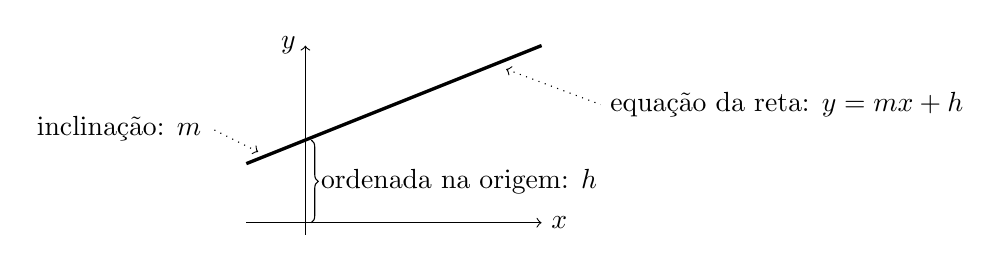
\begin{tikzpicture}[scale=1.5]
\draw [ ->] (0,-0.1)--(0,1.5) node[left]{$y$};
\draw [ ->] (-0.5,0)--(2,0) node[right]{$x$};
\draw [very thick] (-0.5,0.5)--(2,1.5);
\draw [decorate, decoration=brace] (0.05,0.7)--(0.05,0) 
node[midway, right]{ordenada na origem: $h$};
\draw [dotted,  <-] (1.7,1.3)--(2.5,1) node[right]{equação da reta: $y=mx+h$};
\draw [dotted,  <-] (-0.4,0.6)--(-0.8,0.8) node[left]{inclinação: $m$};
\end{tikzpicture}\end{bmlimage}
\end{center}
 O significado da inclinação $m$ deve ser entendido da seguinte maneira: partindo de um
ponto qualquer da reta, ao andar horizontalmente uma distância $L$ para a direita, o
deslocamento vertical da reta é de $mL$. Por exemplo, para uma reta de inclinação
$\frac12$ (observe que todo os triângulos da seguinte figura são semelhantes),
\begin{center}
\begin{bmlimage}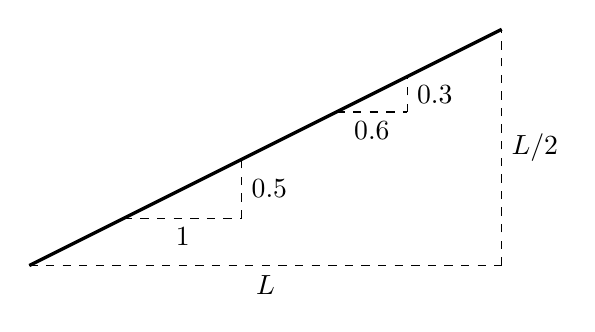
\begin{tikzpicture}[scale=1.5]
\draw [very thick] (0,0)--(4,2);
\draw [dashed] (0,0)--(4,0) node[midway, below]{$L$};
\draw [dashed] (4,0)--(4,2) node[midway, right]{$L/2$};
\draw [dashed] (0.8,0.4)--(1.8,0.4) node[midway, below]{$1$};
\draw [dashed] (1.8,0.4)--(1.8,0.9) node[midway, right]{$0.5$};
\draw [dashed] (2.6,1.3)--(3.2,1.3) node[midway, below]{$0.6$};
\draw [dashed] (3.2,1.3)--(3.2,1.6) node[midway, right]{$0.3$};
\end{tikzpicture}\end{bmlimage}
\end{center}
Se a inclinação é negativa, então o deslocamento vertical é para baixo.\\

 Se $P=(x_1,y_1)$ e $Q=(x_2,y_2)$ 
 são dois pontos de uma reta não vertical de inclinação $m$, então
\eq{\label{eq:exprinclin}
\frac{y_2-y_1}{x_2-x_1}=m\,.}
Essa relação pode ser usada também para \emph{calcular} a inclinação de uma reta. 

\begin{ex}\label{exemploreta}
 Procuremos a equação da reta $r$ que passa pelos pontos $P=(-1,3)$ e $Q=(3,0)$:
\begin{center}
\begin{bmlimage}\begin{tikzpicture}[scale=0.8]
\draw [ ->] (0,-0.1)--(0,3.2) node[right]{$y$};
\draw [ ->] (-1.5,0)--(3.5,0) node[right]{$x$};
\pgfmathsetmacro{\a}{-1.2}
\pgfmathsetmacro{\b}{3.2}
\draw [dotted] (\a,{(-3*\a)/4+9/4})--(\b,{(-3*\b)/4+9/4});
\draw (-1,3) node[below left]{$P$};
\fill (-1,3) circle (0.35mm);
\draw (3,0) node[above]{$Q$};
\fill (3,0) circle (0.35mm);
\foreach \k in {-1,...,3}
{\draw ({\k},0) node{$\shortmid$};}
\foreach \k in {0,...,3}
{\draw (0,{\k}) node{$-$};}
\end{tikzpicture}\end{bmlimage}
\end{center}
Como $r$ não é vertical, a sua equação é da forma $y=mx+h$. A 
inclinação pode ser
calculada usando \eqref{eq:exprinclin}:
$m=\frac{0-(3)}{3-(-1)}=-\frac{3}{4}$.
 (Pode também observar que para andar de $P$ até $Q$, é necessário andar 
$4$ passos para a
direita, e $3$ passos para baixo, logo $m=\tfrac{-3}{4}$.)
 Portanto, a equação é da forma $y=-\tfrac{3}{4}x+h$. Falta achar $h$, 
que pode ser
calculado usando o fato de $r$ passar pelo ponto $P$: 
$3=-\tfrac{3}{4}\cdot (-1)+h$ (daria
na mesma usando o ponto $Q$). 
Assim, $h=\tfrac{9}{4}$, e $r$ é descrita pela equação: $$y=-\tfrac{3}{4}x+\tfrac94\,.$$
 Ao multiplicarmos ambos lados por $4$ e rearranjando podemos a equação da reta
 da seguinte maneira:
$$
3x+4y-9=0\,.
$$
Essa é a \grasA{forma genérica} da reta. 
Em geral, qualquer reta pode ser
descrita na forma  générica,
\[
ax+by+c=0\,,
\]
em que $a,b,c$ são constantes. Se $a=0$ e $b\neq 0$, a reta é horizontal. Se
$a\neq 0$ e $b=0$, a reta é vertical. Se $a\neq 0$ e $b\neq 0$, a reta é oblíqua.

\end{ex}

\begin{exo}
Considere a reta $r$ do Exemplo \ref{exemploreta}.
Escolha alguns pares de pontos $P$ e $Q$ em $r$, 
e verifique a fórmula \eqref{eq:exprinclin}.
Ache os valores de $x$ e $y$ para que os pontos $R=(x,100)$ e $T=(6,y)$ pertençam a $r$.
\begin{sol}
$R=(-\frac{391}{3},100)$, $T=(6,-\frac{9}{4})$.
\end{sol}
\end{exo}

\begin{exo}
Determine a equação da reta que passa pelos pontos dados.
\begin{multicols}{2}
\begin{enumerate}
\item\label{itreta1} $(0,0)$, $(1,1)$
\item\label{itreta2} $(-2,1)$, $(100,1)$
\item\label{itreta3} $(-3,-21.57)$, $(-3,3)$ 
\item\label{itreta4} $(1,-2)$, $(-1,3)$ 
\item\label{itreta5} $(333,227)$, $(-402,-263)$ 
\end{enumerate}
\end{multicols}
\vspace{0.01cm}
\begin{sol}
\eqref{itreta1} $y=x$,
\eqref{itreta2} $y=1$,
\eqref{itreta3} $x=-3$,
\eqref{itreta4} $y=-\tfrac{5}{2}x+\tfrac12$,
\eqref{itreta5} $y=\tfrac{2}{3}x+5$.
\end{sol}
\end{exo}

\begin{exo}\label{ExoEsbocoretas}
Faça um esboço, no plano cartesiano, da reta descrita pela equação dada.
\begin{multicols}{3}
\begin{enumerate}
\item\label{itretta1} $r_1:\,x=4$
 \item\label{itretta2} $r_2:\,y=-3/2$
\item \label{itrett3} $r_3:\,x+2y=0$
\item \label{itrett4} $r_4:\,y=2x-3$
\end{enumerate}
\end{multicols}
\vspace{0.01cm}
\begin{sol}

\mbox{}
\begin{center}
\begin{bmlimage}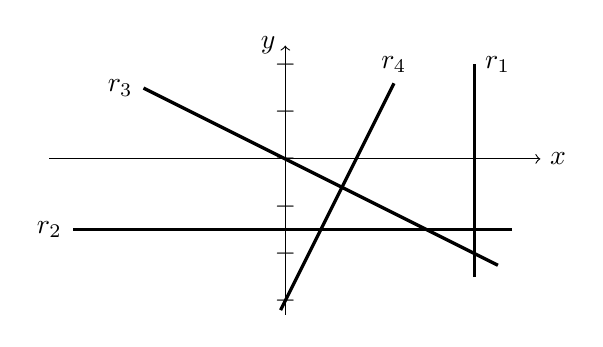
\begin{tikzpicture}[scale=0.6]
\draw [ ->] (0,-3.3)--(0,2.4) node[left]{$y$};
\draw [ ->] (-5,0)--(5.4,0) node[right]{$x$};
\foreach \k in {-5,...,5}
{\draw ({\k},0) node{$\shortmid$};}
\foreach \k in {-3,...,2}
{\draw (0,{\k}) node{$-$};}
%%%%%%%%
\draw [very thick] (4,-2.5)--(4,2) node[right]{$r_1$};
%%%%%%%%%%%%
%\draw (4.2,0.2) node{$4$};
\draw [very thick] (4.8,-1.5)--(-4.5,-1.5) node[left]{$r_2$};
%\draw (0,-1.5) node[above left]{$-\tfrac{3}{2}$};
%%%%%%%%%%%%
%\draw (4.2,0.2) node{$4$};
\pgfmathsetmacro{\a}{-0.1}
\pgfmathsetmacro{\b}{2.3}
\draw [very thick] (\a,{(2*\a)-3})--(\b,{2*\b-3}) node[above]{$r_4$};
%%%
\pgfmathsetmacro{\c}{-3}
\pgfmathsetmacro{\d}{4.5}
\draw [very thick] (\d,{(-\d)/2})--(\c,{(-\c)/2}) node[left]{$r_3$};
\end{tikzpicture}\end{bmlimage}
\end{center}
\end{sol}
\end{exo}

Observe que retas paralelas têm a mesma inclinação.

\begin{exo}
Dê a equação da reta $r'$, paralela a $r$, que passa pelo ponto $P$.
\begin{multicols}{2}
 \begin{enumerate}
  \item\label{ittexreta1} $r:\,y=5x+2$, $P=(-1,5)$.
\item\label{ittexreta2} $r:\,4x-3y+6=0$, $P=(3,-5)$.
 \end{enumerate}
\end{multicols}
\vspace{0.01cm}
\begin{sol}
\eqref{ittexreta1} $r':\,y=5x+10$.
\eqref{ittexreta2} $r':\,y=\tfrac{4}{3}x-9$
\end{sol}
\end{exo}

\begin{exo}
Mostre que se $r_1$ tem inclinação $m_1\neq 0$, e $r_2$ tem inclinação
$m_2=-\frac{1}{m_1}$, então $r_1$ e $r_2$ são perpendiculares.
 \begin{sol} Comecemos com um exemplo: considere a reta $r_1$ de inclinação $m_1=\tfrac13$
que passa pela origem. Qual é a equação da reta $r_2$, perpendicular a $r_1$, que passa
pela origem?
\begin{center}
 \begin{bmlimage}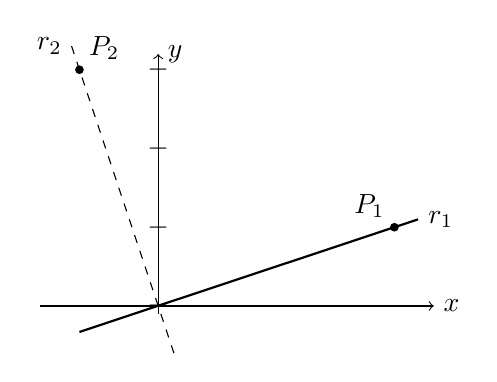
\begin{tikzpicture}
  \draw [ ->] (0,-0.1)--(0,3.2) node[right]{$y$};
\draw [ ->] (-1.5,0)--(3.5,0) node[right]{$x$};
\draw[thick] (-1,-0.33)--(3.3,1.1) node[right]{$r_1$};
\draw[dashed] (0.2,-0.6)--(-1.1,3.3) node[left]{$r_2$};
\fill (3,1) circle (0.55mm);
\draw (3,1) node[above left]{$P_1$};
\fill (-1,3) circle (0.55mm);
\draw (-1,3) node[above right]{$P_2$};
\foreach \k in {-1,...,3}
{\draw ({\k},0) node{$\shortmid$};}
\foreach \k in {0,...,3}
{\draw (0,{\k}) node{$-$};}
 \end{tikzpicture}\end{bmlimage}
\end{center}
 Observe que se $P_1=(3,1)\in r_1$, então o ponto $P_2=(-1,3)\in r_2$, já que o segmento
$OP_1$ precisa ser perpendicular a $OP_2$. Logo, a inclinação de $r_2$ pode ser obtida
usando o ponto $P_2$:
$m_2=\frac{0-3}{0-(-1)}=-3$,
 o que prova $m_2=-\frac{1}{m_1}$. Escolhendo qualquer outro ponto $P_1=(x,y)$ em $r_1$,
obteríamos um ponto $P_2=(-y,x)$, e $m_2$ seria calculada da mesma maneira.\\

 Para uma reta de inclinação $m_1$ qualquer, podemos escolher $P_1=(1,m_1)$ e
$P_2=(-m_1,1)$, assim $m_2=\frac{0-1}{0-(-m_1)}=-\frac{1}{m_1}$ é sempre verificada.
\end{sol}
\end{exo}

\begin{exo}
Determine quais das seguintes retas são paralelas ou perpendiculares.
$$r_1:\,2x+y-1=0\,,\quad r_2:\,x+2y+1=0\,,\quad r_3:\,y=2x-3\,,\quad r_4:\,3x+6y-3=0\,.$$
Em seguida, esboce as retas e verifique.
\begin{sol}
$r_2$ e $r_4$ são paralelas, e ambas são perpendiculares a $r_3$.
\end{sol}
\end{exo}

\subsection{Círculos}\label{SecCirculos}\index{círculo}

Considere o círculo~\footnote{Às vezes, o que chamamos aqui de \emph{círculo} corresponde
a \emph{circunferência} em outros textos de matemática elementar.} $\gamma$ de centro
$C=(1,2)$ e de raio $R=2$:
\begin{center}
\begin{bmlimage}\begin{tikzpicture}[scale=0.6]
\draw [ ->] (0,-1)--(0,4.4) node[left]{$y$};
\draw [ ->] (-2,0)--(4,0) node[right]{$x$};
\foreach \k in {-2,...,3}
{\draw ({\k},0) node{$\shortmid$};}
\foreach \k in {-1,...,4}
{\draw (0,{\k}) node{$-$};}
\draw (3,2) arc (0:360:2);
\fill (1,2) circle (0.55mm);
\draw (1,2) node[above right]{$C$};
\draw (2.8,3.8) node{$\gamma$};
\end{tikzpicture}\end{bmlimage}
\end{center}
 Por definição (ver o Exercício \ref{Exo:subconjplano}), $\gamma$ é definido pelo conjunto
dos pontos $P$ cuja distância euclidiana a $C$ é igual a $2$:
 $d(P,C)=2$. Isso significa que as coordenadas $(x,y)$ de $P$ são ligadas pela seguinte
expressão:
$\sqrt{(x-1)^2+(y-2)^2}=2$. Equivalentemente, $\gamma$ é descrito pela seguinte equação:
$${(x-1)^2+(y-2)^2}=4\,.$$
 Observe que, expandindo os fatores $(x-1)^2$ e $(y-2)^2$, essa última expressão pode ser
escrita na \grasA{forma genérica}\index{círculo! forma genérica}:
$$x^2+y^2-2x-4y+1=0\,.$$

Em geral, um círculo de raio $R>0$ centrado em $C=(x_0,y_0)$ é descrito pela equação
\eq{(x-x_0)^2+(y-y_0)^2=R^2\,.}
Um problema clássico é de achar o centro e o raio a partir da forma genérica.
\begin{ex}
Considere o círculo $\gamma$ descrito pela sua equação genérica 
\eq{\label{eqcirgenerica}
x^2+y^2+6x-8y=0\,.}
Para achar o seu centro e o seu raio, completemos os quadrados\index{completar um
quadrado}: $x^2+6x=(x+3)^2-9$, $y^2-8y=(y-4)^2-16$. Logo, 
\eqref{eqcirgenerica} pode ser escrita como
$(x+3)^2-9+(y-4)^2-16=0$, isto é:
$$(x+3)^2+(y-4)^2=25\equiv 5^2\,.$$
Portanto, $\gamma$ é centrado em $C=(-3,4)$, de raio $R=5$.
\end{ex}

\begin{ex}
Considere $x^2+2x+y^2+2=0$. Completando o quadrado e rearranjando, obtemos
$(x+1)^2+y^2=-1$. Como ``$-1$'' não pode ser escrito como um quadrado, esta equação
não representa um círculo (e na verdade, não existe nenhum par $(x,y)$ que seja
solução).
\end{ex}

\begin{exo}
Determine quais das equações a seguir definem um círculo. Quando for o caso, calcule 
o centro e o raio.
\begin{multicols}{3}
\begin{enumerate}
\item\label{itexcirc1} $x^2+(y+1)^2=9$
\item\label{itexcirc2} $x^2+y^2=-1$
\item\label{itexcirc3} $x^2+y^2=6x$
\item\label{itexcirc4} $x^2+y^2+x+y+1=0$
\item\label{itexcirc5} $x^2+y^2+2x+1=0$
\item\label{itexcirc6} $x^2=y^2+1$
\end{enumerate}
\end{multicols}
\vspace{0.01cm}
\begin{sol}
\eqref{itexcirc1} $C=(0,-1)$, $R=3$.
\eqref{itexcirc2} não é círculo: $-1$ não é um quadrado.
\eqref{itexcirc3} $C=(3,0)$, $R=3$.
 \eqref{itexcirc4} não é círculo: depois de ter completado o quadrado obtemos
$(x+\half)^2+(y+\half)^2=-\half$, que não é um quadrado.
 \eqref{itexcirc5} não é círculo: depois de ter completado o quadrado obtemos
$(x+1)^2+y^2=0$ (que poderia ser interpretado como um círculo de raio $R=0$ centrado em
$(-1,0)$).
\eqref{itexcirc6} não é círculo ($x^2-y^2=1$ é
uma \emph{hipérbole}).
\end{sol}
\end{exo}

\section{Trigonometria}\index{trigonometria}                                  
A \emph{trigonometria} estabelece relações precisas entre os ângulos e os
lados de um triângulo.
Definiremos as três funções (mesmo se a própria noção de \emph{função}
será estudada no próximo capítulo) 
trigonométricas elementares, $\sen$ (seno), $\cos$ (cosseno) e $\tan$ (tangente), e
daremos as suas propriedades básicas. Nos próximos capítulos olharemos
mais de perto as propriedades analíticas dessas funções.
    
\subsection{Medir ângulos no plano}\index{ângulo}

 Para começar, é importante escolher uma \emph{unidade} (como ``metros'' para
comprimentos, ou ``litros'' para volumes) para medir um ângulo
determinado pela abertura entre duas retas.
Descreveremos as duas unidades mais usadas, \emph{graus} e \emph{radianos}.\\

Os ângulos serão medidos a partir de uma reta horizontal, em sentido
\emph{antihorário}.  A abertura mínima, naturalmente, é definida como
valendo zero, qualquer que seja a unidade.
O que precisa ser definido é o valor do \emph{ângulo total}.
Se o ângulo for medido em \grasA{graus}\index{ângulo! medido em graus}, 
esse ângulo total é definido como valendo \grasA{$360$ graus}:
\begin{center}
\begin{bmlimage}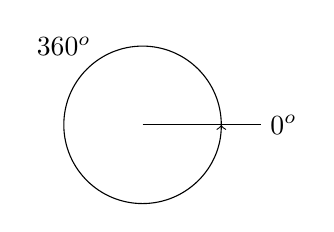
\begin{tikzpicture}[scale=1]
\draw (0,0)--(1.5,0) node[right]{$0^o$};
\draw[ ->] (1,0) arc (0:360:1);
\draw (-1,1) node{$360^o$};
\end{tikzpicture}\end{bmlimage}
\end{center}
 Uma vez que o ângulo total foi fixado, a medição dos outros se faz proporcionalmente: a
metade do ângulo total vale $180$ graus, o ângulo reto mede $90$ graus, etc.
A vantagem dessa unidade é que vários ângulos bastante usados em geometria tomam valores
inteiros: $30$, $60$, $90$, $180$, $270$, etc.
\begin{center}                                                                          
\begin{bmlimage}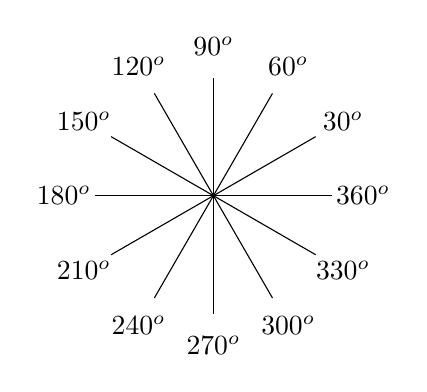
\begin{tikzpicture}[scale=1]
\foreach \k in {30,60,90,120,150,180,210,240,270,300,330,360}
{
\draw (0,0)--({\k}:1.5);
\draw ({\k}:1.9) node{$\k^o$};
}
\end{tikzpicture}\end{bmlimage}
\end{center}
Observe que apesar da posição do ângulo total coincidir com o ângulo
nulo, eles devem ser considerados como distintos.\\

Fixar o ângulo total como sendo igual a $360$ pode parecer arbitrário,
e um jeito mais natural de definir o ângulo total é de usar a
noção de comprimento usual na reta.
De fato, considere o 
círculo de raio $1$ centrado na origem e, partindo do ponto $(1,0)$ (que corresponde
a um ângulo de $0$), 
ande ao longo do círculo no sentido antihorário. Quando tiver
percorrido uma distância igual ao raio do círculo, o ângulo
correspondente é definido como sendo de \grasA{$1$ (um)
radiano}\index{ângulo! medido em radianos}: 

 \begin{center}
 \begin{bmlimage}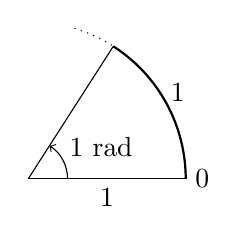
\begin{tikzpicture}[scale=1]
\draw (0,0)--(2,0) node[right]{$0$};
\draw[dotted] (2,0) arc (0:73:2);
\draw(0,0)--(1 r:2);
\draw (0,0)--(2,0) node[midway, below]{$1$};
\draw (1.9,1.1) node{$1$};
\draw[thick]  (2,0) arc (0:1 r:2);
\draw[ ->] (0.5,0) arc (0:1 r:0.5);
\draw (0.4,0.4) node[right]{$1$ rad};
\end{tikzpicture}\end{bmlimage}
 \end{center}
Observe que o ângulo total corresponde à circunferência de um círculo de raio $1$:
$2\pi$.\\


 Em geral, nessa apostila, os ângulos serão medidos em radianos. Se a medida de um ângulo
em graus é $\alpha_g$ e em radianos é $\alpha_r$,
 a conversão se faz da seguinte maneira: como o ângulo total mede $360$ graus e $2\pi$
radianos, temos $\frac{360}{2\pi}=\frac{\alpha_g}{\alpha_r}$. Portanto,
\eq{
\alpha_g=\frac{180}{\pi}\alpha_r\,,\quad\text{ ou   }
\alpha_r=\frac{\pi}{180}\alpha_g\,.}
Assim, verifica-se por exemplo que um ângulo de $90$ graus corresponde a
$\frac{\pi}{180}90=\tfrac{\pi}{2}=1.57...$ radianos.

\begin{exo} O ponteiro dos segundos de um relógio mede $20$ 
centímetros. Qual distância a
ponta desse ponteiro percorreu depois de uma hora e 15 minutos?
 \begin{sol} Durante uma hora e quinze minutos, o ponteiro dos segundos 
dá $75$ voltas.
Como uma volta representa uma distância percorrida (pela ponta) de 
$2\times \pi\times
20\simeq 125.66$ centímetros, a distância total é de $\simeq 9424.5$ 
centímetros, o que corresponde a $\simeq 94.25$ metros.
\end{sol}
\end{exo}

\begin{exo}
Estime a velocidade (em km/s) com a qual a lua gira em torno 
da terra, sabendo que a distância média terra-lua fica é de 384'400km
e que uma volta dura aproximadamente um mês.
\end{exo}

Um ângulo \emph{negativo} será interpretado como medido no sentido horário:
\begin{center}
\begin{bmlimage}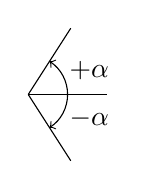
\begin{tikzpicture}[scale=1]
\pgfmathsetmacro{\a}{2.3};
\draw(0,0)--(1 r:1);
\draw(0,0)--(-1 r:1);
\draw (0,0)--(1,0);
\draw[ ->] (0.5,0) arc (0:1 r:0.5);
\draw (0.4,0.3) node[right]{$+\alpha$};
\draw[ ->] (0.5,0) arc (0:-1 r:0.5);
\draw (0.4,-0.3) node[right]{$-\alpha$};
\end{tikzpicture}\end{bmlimage}
\end{center}

\subsection{Seno, cosseno e tangente}
Para poder definir as ligações entre os ângulos e os lados de um triângulo, é necessário 
fazer umas simplificações. Trabalharemos com um \grasA{triângulo retângulo}, 
isto é, que possui um ângulo reto. Considere então o seguinte triângulo $ABC$, retângulo
em $C$:
\begin{center}
\begin{bmlimage}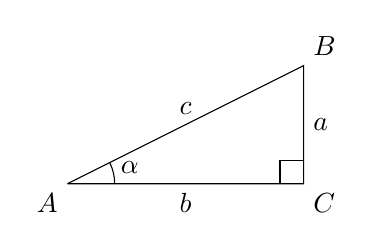
\begin{tikzpicture}[scale=1.5]
\draw (0,0)--(2,1) node[midway, above]{$c$} node[above right]{$B$}--(2,0) 
node[midway, right]{$a$} node[below right]{$C$} --(0,0) node[midway,
below]{$b$}node[below left]{$A$};
\draw (0.4,0) arc (0:26.56:0.4);
\draw (1.8,0)--(1.8,0.2)--(2,0.2);
\draw (0.37,0) node[above right]{$\alpha$};
%\draw (2.8,3.8) node{$\gamma$};
\end{tikzpicture}\end{bmlimage}
\end{center}
Com respeito a $\alpha$, $b$ é chamado de \grasA{cateto adjacente}, $a$ de 
\grasA{cateto oposto}, e $c$ de \grasA{hipotenusa}.\\

 Se dois lados forem conhecidos, o terceiro pode ser calculado usando o Teorema de
Pitágoras, e  o valor do ângulo $\alpha$ é determinado.
Como qualquer triângulo semelhante a $ABC$ tem os mesmos ângulos, $\alpha$ é
determinado uma vez que um dos quocientes $\tfrac{a}{c}$, $\tfrac{b}{c}$, ou
$\tfrac{a}{b}$ for conhecido. A ligação entre $\alpha$ e esses quocientes é
chamada respectivamente
\grasA{seno, cosseno e tangente de $\alpha$}, e
denotada\index{seno}\index{cosseno}\index{tangente} por
$$\boxed{\sen \alpha\pardef \frac{a}{c}\,,\quad 
\cos \alpha\pardef \frac{b}{c}\,,\quad 
\tan \alpha\pardef \frac{a}{b}\,.}$$
(Aqui escreveremos a tangente $\tan \alpha$, mas às vezes se encontra
também a notação $\mathrm{tg}\,\alpha$.)
Observe que a seguinte relação sempre vale:
\eq{\label{eqtrigo1}
\tan \alpha=\frac{\sen \alpha}{\cos \alpha}}
Em alguns casos simples, $\sen \alpha$, $\cos \alpha$ e $\tan \alpha$ podem ser
calculados ``manualmente''. 
\begin{ex} Considere $\alpha=\tfrac{\pi}{4}$ ($=45^o$). Para calcular 
$\sen \tfrac{\pi}{4}$, $\cos \tfrac{\pi}{4}$ e $\tan \tfrac{\pi}{4}$, 
consideremos o seguinte triângulo:
\begin{center}
\begin{bmlimage}\begin{tikzpicture}[scale=1.5]
 \draw (0,0)--(1,0) node[midway, below, color=\coulcoseno]{$1$} --(1,1) node[midway,
right, color=\coulseno]{$1$} --(0,0) node[midway, above left]{$\sqrt{2}$};
\draw (0.4,0) arc (0:45:0.4);
\draw (0.35,0) node[above right]{$\tfrac{\pi}{4}$};
 \draw (2,0.5) node[right]{$\Rightarrow\,\sen
\tfrac{\pi}{4}=\frac{\textcolor{\coulseno}{1}}{\sqrt{2}}\,, \quad
 \cos \tfrac{\pi}{4}=\frac{\textcolor{\coulcoseno}{1}}{\sqrt{2}}\,,\quad\tan
\tfrac{\pi}{4}=\tfrac{\textcolor{\coulseno}{1}}{\textcolor{\coulcoseno}{1}}=1$\,.};
\end{tikzpicture}\end{bmlimage}
\end{center}
\end{ex}

\begin{exo}\label{exo:calculsimple60} Montando em cada caso um triângulo apropriado,
calcule (sem calculadora) $\sen \tfrac{\pi}{3}$, $\cos \tfrac{\pi}{3}$,
$\tan \tfrac{\pi}{3}$, $\sen \tfrac{\pi}{6}$, $\cos \tfrac{\pi}{6}$,
$\tan \tfrac{\pi}{6}$. 
\begin{sol}
\mbox{}

\begin{center}
\begin{bmlimage}\begin{tikzpicture}[scale=2]
 \draw (0,0)--(0.5,0) node[midway, below]{$\tfrac12$} --(0.5,0.866)--(0,0) node[midway,
above left]{$1$};
\draw (0.6,0.35) node{$\frac{\sqrt{3}}{2}$};
\draw (0.225,0.15) node{$\tfrac{\pi}{3}$};
\draw (0.2,0) arc (0:60:0.2);
\draw (0.4,0.5) node{$\tfrac{\pi}{6}$};
\draw (0.4,0.7) arc (240:265:0.25);
\draw (1.5,0.7) node[right]{$\Rightarrow\,\sen \tfrac{\pi}{3}=\frac{\sqrt{3}}{{2}}\,, \quad
\cos \tfrac{\pi}{3}=\frac{1}{{2}}\,,\quad \tan \tfrac{\pi}{3}=\sqrt{3}$\,.};
\draw (1.5,0.2) node[right]{$\Rightarrow\,\sen \tfrac{\pi}{6}=\frac{1}{{2}}\,, \quad
 \cos \tfrac{\pi}{6}=\frac{\sqrt{3}}{{2}}\,,\quad \tan
\tfrac{\pi}{6}=\tfrac{1}{\sqrt{3}}$\,.};
\draw[dotted] (0.5,0)--(1,0)--(0.5,0.866)--cycle;
\end{tikzpicture}\end{bmlimage}
\end{center}
\end{sol}
\end{exo}

\begin{exo}
Para determinar a altura $H$ de uma torre, 
ficamos a uma distância qualquer dela, e medimos o ângulo $\alpha$
entre a horizontal e o topo da torre. Em seguida, andamos uma distância
$d$ em direção à base da torre, e medimos o ângulo $\beta$
entre a horizontal e o topo da torre. 
Expresse $H$ como função de $\alpha,\beta,d$.
\begin{sol}
$H=\frac{d(\tan\beta-\tan\alpha)}{\tan \alpha\tan\beta}$.
\end{sol}
\end{exo}

Faremos agora uma generalização, que permitirá 
\emph{enxergar} melhor os três números $\sen \alpha$, $\cos \alpha$ e 
$\tan \alpha$,  e
que será também útil para considerá-las como \emph{funções de uma 
variável real}, a partir do próximo capítulo.\\

Para tanto, usaremos um triângulo cuja hipotenusa é de tamanho $c=1$. 
Isto é, o ponto $B$
do triângulo da
figura acima é posicionado no círculo de raio $1$ centrado na origem, 
chamado
\grasA{círculo trigonométrico}\index{círculo trigonométrico}. As funções 
trigonométricas
podem então ser medidas efetivamente olhando para os comprimentos da 
seguinte figura:

\begin{center}
\begin{bmlimage}\begin{tikzpicture}[scale=1]
\pgfmathsetmacro{\a}{2.3};
\draw (-\a,0) -- (0,0);
\draw[ ->] (0,-\a) -- (0,\a);
\draw[ ->] (1.1,0)-- (\a,0);
 \draw [color=\coulseno, thick] (1.1,1.665)--(1.1,0) node[midway, above, sloped]{$\sen
\alpha$};
\draw [color=\coultang, thick] (2,3)--(2,0) node[midway, above, sloped]{$\tan \alpha$};
\draw [color=\coulcoseno, thick] (1.1,0)--(0,0) node[midway, below]{$\cos \alpha$};
\draw (1.1,1.665) node[above]{$B$};
\draw[dotted] (2,0) arc (0:360:2);
\draw(0,0)--(2,3);
%\draw (0,0)--(2,0);
\draw (0.5,1.1) node{$1$};
\draw[ ->] (0.5,0) arc (0:1 r:0.5);
\draw (0.4,0.3) node[right]{$\alpha$};
\fill (1.1,1.665) circle (0.45mm);
\end{tikzpicture}\end{bmlimage}
\end{center}

 Observe como $\sen \alpha$, $\cos \alpha$ e $\tan \alpha$ mudam à 
medida que $B$ se
movimenta ao longo do círculo. Em particular, $B$ pode dar uma volta 
completa no círculo,
o que permite estender as funções trigonométricas a qualquer
ângulo~\footnote{A tangente tem um problema nos múltiplos de
$\pisobredois$ (ver mais adiante).} 
$0\leq \alpha \leq 2\pi$, e também para valores maiores ou até negativos. 
Os sinais das funções trigonométricas mudam dependendo do quadrante ao qual $B$ pertence:

\begin{center}
\begin{bmlimage}\begin{tikzpicture}[scale=1]
\pgfmathsetmacro{\a}{2.1};
\draw[ ->] (-\a,0) -- (\a,0);
\draw[ ->] (0,-\a) -- (0,\a);
\draw[right] (0,1.8) node{$1^o:$};
\draw[color=\coulseno,right] (0,1.3) node{$\sen \alpha\geq 0$};
\draw[color=\coulcoseno,right] (0,0.8) node{$\cos \alpha\geq 0$};
\draw[color=\coultang,right] (0,0.3) node{$\tan \alpha\geq 0$};

\pgfmathsetmacro{\a}{-2.1};
\draw[right] (\a,1.8) node{$2^o:$};
\draw[color=\coulseno,right] (\a,1.3) node{$\sen \alpha\geq 0$};
\draw[color=\coulcoseno,right] (\a,0.8) node{$\cos \alpha\leq 0$};
\draw[color=\coultang,right] (\a,0.3) node{$\tan \alpha\leq 0$};

\pgfmathsetmacro{\h}{2.1}
\draw[right] (\a,1.8-\h) node{$3^o:$};
\draw[color=\coulseno,right] (\a,1.3-\h) node{$\sen \alpha\leq 0$};
\draw[color=\coulcoseno,right] (\a,0.8-\h) node{$\cos \alpha\leq 0$};
\draw[color=\coultang,right] (\a,0.3-\h) node{$\tan \alpha\geq 0$};

\draw[right] (0,1.8-\h) node{$4^o:$};
\draw[color=\coulseno,right] (0,1.3-\h) node{$\sen \alpha\leq 0$};
\draw[color=\coulcoseno,right] (0,0.8-\h) node{$\cos \alpha\geq 0$};
\draw[color=\coultang,right] (0,0.3-\h) node{$\tan \alpha\leq 0$};
\end{tikzpicture}\end{bmlimage}
\end{center}

Várias propriedades podem ser obtidas a partir do círculo trigonométrico. Por exemplo, 
 observe que $\alpha$ e $-\alpha$ têm o mesmo cosseno, mas que ao transformar $\alpha$ em
$-\alpha$, o seno muda de sinal. Portanto,
\eq{\label{eqtrigo0}
\cos(-\alpha)=\cos\alpha\,,\quad
\sen(-\alpha)=-\sen\alpha\,,\quad
\tan(-\alpha)=-\tan\alpha\,.}

Todas as identidades do seguinte exercício podem ser obtidas de maneira
parecida, olhando simplesmente para o círculo trigonométrico.

\begin{exo}\label{exorelattrigo}\index{identidades trigonométricas}
Prove as identidades:
\eq{\label{eqtrigo00}
\cos(\pi-\alpha)=-\cos\alpha\,,\quad
\sen(\pi-\alpha)=\sen\alpha\,,\quad
\tan(\pi-\alpha)=-\tan\alpha\,.}
\eq{\label{eqtrigo000}
\cos(\pi+\alpha)=-\cos\alpha\,,\quad
\sen(\pi+\alpha)=-\sen\alpha\,,\quad
\tan(\pi+\alpha)=\tan\alpha\,.}
\eq{\label{eqtrigo0000}
\cos(\tfrac{\pi}{2}-\alpha)=\sen\alpha\,,\quad
\sen(\tfrac{\pi}{2}-\alpha)=\cos\alpha\,,\quad
\tan(\tfrac{\pi}{2}-\alpha)={\cot\alpha}\,.}
\eq{\label{eqtrigo00000}
\cos(\tfrac{\pi}{2}+\alpha)=-\sen\alpha\,,\quad
\sen(\tfrac{\pi}{2}+\alpha)=\cos\alpha\,,\quad
\tan(\tfrac{\pi}{2}+\alpha)=-{\cot\alpha}\,.}
 A \grasA{cotangente}, definida por $\cot \alpha\pardef \frac{1}{\tan \alpha}$, apareceu
naturalmente.
\begin{sol} 
Todas essas identidades seguem da observação do círculo trigonométrico. Por exemplo, 
o desenho
\begin{center}
\begin{bmlimage}\begin{tikzpicture}[scale=3]
\pgfmathsetmacro{\a}{1};
\draw[dotted] (\a,0) arc (0:180:\a);
\draw[ ->, color=gray!70] (-1.1*\a,0) -- (1.1*\a,0);
\draw[ ->, color=gray!70] (0,0) -- (0,1.1*\a);

\pgfmathsetmacro{\alf}{35};

%DESSINER LES ANGLES:
\draw[ ->] ({0.4*\a},0) arc (0:\alf:{0.4*\a});
%\draw ({(\alf)/2}:{(\a)*(0.45)}) node{$\alpha$};
\draw ({\alf/2}:{\a*0.45}) node{$\alpha$};
\draw[ ->] ({0.3*\a},0) arc (0:180-\alf:{0.3*\a});
\draw ({(180-\alf)/2}:{0.35*\a}) node[above]{$\pi-\alpha$};

%DEFINIR LES POINTS:
\coordinate (B) at ({\a*cos(\alf)},{\a*sin(\alf)});
\draw (B) node[above right]{$B$};
\fill (B) circle (0.15 mm);
\draw (0,0)--(B);

\coordinate (C) at ({\a*cos(180-\alf)},{\a*sin(180-\alf)});
%\draw (C) node[above left]{$C$};
\fill (C) circle (0.15 mm);
\draw (0,0)--(C);

\draw[dotted] (C)--(B);

 \draw [color=\coulseno, thick] (B)--({\a*cos(\alf)},0) node[midway, above, sloped]{$\sen
\alpha$};
 \draw [color=\coulcoseno, thick] ({\a*cos(\alf)},0)--(0,0) node[midway, below]{$\cos
\alpha$};
 \draw [color=\coulseno, thick] (C)--({\a*cos(180-\alf)},0) node[midway, above,
sloped]{$\sen (\pi-\alpha)$};
 \draw [color=\coulcoseno, thick] ({\a*cos(180-\alf)},0)--(0,0) node[midway, below]{$\cos
(\pi-\alpha)$};

\end{tikzpicture}\end{bmlimage}
\end{center}
mostra que $\cos(\pi-\alpha)=-\cos\alpha$ e $\sen(\pi-\alpha)=\sen\alpha$.
 Como consequência, 
$$\tan(\pi-\alpha)=\frac{\sen(\pi-\alpha)}{\cos(\pi-\alpha)}=-\tan \alpha\,.$$
Deixemos o leitor provar as identidades parecidas com $\pi+\alpha$.
Por outro lado, o desenho
\begin{center}
\begin{bmlimage}\begin{tikzpicture}[scale=3]
\pgfmathsetmacro{\a}{1};
\draw[dotted] (\a,0) arc (0:90:\a);
\draw[ ->, color=gray!70] (0,0) -- (1.1*\a,0);
\draw[ ->, color=gray!70] (0,0) -- (0,1.1*\a);

\pgfmathsetmacro{\alf}{35};

%DESSINER LES ANGLES:
\coordinate (P) at ({0.4*\a*cos(\alf)},{0.4*\a*sin(\alf)});
\draw[ <-] (P) arc (\alf:90:{0.4*\a});
\draw[ ->] ({0.4*\a},0) arc (0:\alf:{0.4*\a});
\draw ({\alf/2}:{0.45*\a}) node{$\alpha$};
\draw ({\alf+(90-\alf)/2}:{0.35*\a}) node[above right]{$\tfrac{\pi}{2}-\alpha$};

%DEFINIR LES POINTS:
\coordinate (B) at ({\a*cos(\alf)},{\a*sin(\alf)});
\coordinate (Bx) at ({\a*cos(\alf)},0);
\coordinate (By) at (0,{\a*sin(\alf)});

\draw (B) node[above right]{$B$};
\draw (0,0)--(B);
\draw [color=\coulseno, thick] (B)--(Bx) node[midway, above, sloped]{$\sen \alpha$};
\draw [color=\coulcoseno, thick] (Bx)--(0,0) node[midway, below]{$\cos \alpha$};
 \draw [color=\coulseno, thick] (By)--(B) node[midway, above,
sloped]{$\sen(\tfrac{\pi}{2}- \alpha)$};
 \draw [color=\coulcoseno, thick] (By)--(0,0) node[midway, below,
sloped]{$\cos(\tfrac{\pi}{2}- \alpha)$};

\fill (B) circle (0.15 mm);
\end{tikzpicture}\end{bmlimage}
\end{center}
 mostra que $\cos(\tfrac{\pi}{2}-\alpha)=\sen\alpha$ e
$\sen(\tfrac{\pi}{2}-\alpha)=\cos\alpha$.
Como consequência,
$$
 \tan
(\tfrac{\pi}{2}-\alpha)=\frac{\sen(\tfrac{\pi}{2}-\alpha)}{\cos(\tfrac{\pi}{2}-\alpha)}=
\frac{\cos\alpha}{\sen\alpha}\equiv \frac{1}{\tan \alpha}=\cot \alpha\,.
$$
\end{sol}
\end{exo}

\begin{exo}
Complete a seguinte tabela
\begin{center}
\begin{tabular}{|c|c|c|c|c|c|c|c|c|c|c|c|c|c|c|}
\hline
graus & $0$ & $30$&$45$&$60$&$90$&$120$&$150$&$180$&$210$&$240$&$270$&$300$&$330$&$360$\\
\hline
 rad &$0$ &$\tfrac{\pi}{6}$
&$\tfrac{\pi}{4}$&$\tfrac{\pi}{3}$&$\tfrac{\pi}{2}$&$\tfrac{2\pi}{3}$&$\tfrac{5\pi}{6}
$&$\pi$&$\tfrac{7\pi}{6}$&$\tfrac{4\pi}{3}$&$\tfrac{3\pi}{2}$&$\tfrac{5\pi}{3}$&$\tfrac{
11\pi}{6}$&$2\pi$\\ \hline
$\sen$ &$0$ & &$\frac{{1}}{\sqrt{2}}$& &$1$&&&$0$&&&&&&$0$\\  \hline
$\cos$ &$1$ & &$\frac{{1}}{\sqrt{2}}$&&$0$&&&$-1$&&&&&&$1$\\ \hline
$\tan$ &$0$ & &$1$&& $\varnothing$ &&&$0$&&&&&&$0$\\
\hline
\end{tabular}
\end{center}
\end{exo}

\subsection{Identidades trigonométricas}\index{identidades trigonométricas}
As identidades do Exercício \ref{exorelattrigo} deram algumas ligações entre 
seno, cosseno e tangente.
O Teorema de Pitágoras dá também a relação
\eq{\label{eqtrigo2}\cos^2\alpha
+\sen^2\alpha=1\,.}
Provaremos agora a identidade
\begin{align}
\sen(\alpha+\beta)&=\sen\alpha\cos\beta+\cos \alpha\sen\beta\,.\label{eqsensoma}
\end{align}
Apesar desta valer para ângulos $\alpha$ e $\beta$ quaisquer, suporemos que 
$\alpha,\beta\in (0,\pisobrequatro)$, 
e usaremos o seguinte desenho:
\begin{center}
\begin{bmlimage}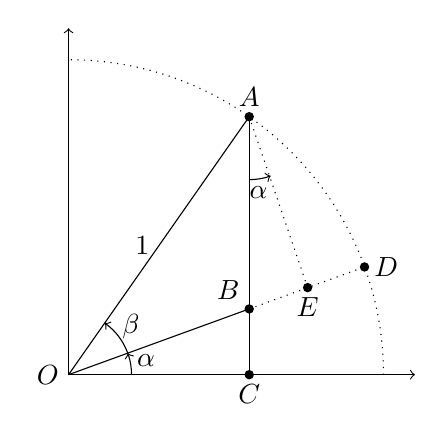
\begin{tikzpicture}[scale=4]
\pgfmathsetmacro{\a}{1};
\draw[dotted] (\a,0) arc (0:90:\a);
\draw[ ->] (0,0) -- (1.1*\a,0);
\draw[ ->] (0,0) -- (0,1.1*\a);

\pgfmathsetmacro{\alf}{20};
\pgfmathsetmacro{\bet}{35};

\draw[ ->] ({0.2*\a},0) arc (0:\alf:{0.2*\a});
\draw ({\alf/2}:{\a/4}) node{$\alpha$};
\draw[ ->] (\alf:{0.2*\a}) arc (\alf:{\alf+\bet}:{0.2*\a});
\draw ({\alf+\bet/2}:{\a/4}) node{$\beta$};

\coordinate (A) at ({\a*cos(\alf+\bet)},{\a*sin(\alf+\bet)});
\coordinate (B) at ({\a*cos(\alf+\bet)},{cos(\alf+\bet)*tan(\alf)});
\coordinate (C) at ({\a*cos(\alf+\bet)},0);
\coordinate (D) at ({\a*cos(\alf)},{\a*sin(\alf)});
\coordinate (E) at ({\a*cos(\alf+\bet)+(sin(\alf)*sin(\bet)/(sqrt(1+(sin(\alf))^2)))},{\a*sin(\alf+\bet)-((sin(\bet))/(sqrt(1+(sin(\alf))^2)))});

\draw (0,0) node[below, left]{$O$};
\pgfmathsetmacro{\ra}{0.15};
\draw (A) node[above]{$A$};
\fill (A) circle (\ra mm);

\fill (B) circle (\ra mm);
\draw (B) node[above left]{$B$};

\fill (C) circle (\ra mm);
\draw (C) node[below]{$C$};

\fill (D) circle (\ra mm);
\draw (D) node[right]{$D$};

\fill (E) circle (\ra mm);
\draw (E) node[below]{$E$};

\draw[ ->] ({\a*cos(\alf+\bet)},{\a*sin(\alf+\bet)-0.2*\a}) arc
(270:{270+\alf}:{0.2*\a});
\draw  ({\a*cos(\alf+\bet)-0.03*\a},{\a*sin(\alf+\bet)-0.24*\a})
node[below, right]{$\alpha$};

\draw (0,0)--(A) node[midway, above, left]{$1$};
\draw (0,0)--(B);
\draw (0,0)--(C);
\draw (A)--(C);
\draw[dotted] (B)--(D);
\draw[dotted] (A)--(E);
\end{tikzpicture}\end{bmlimage}
\end{center}
Observe que $\sen(\alpha+\beta)=d(A,C)=d(A,B)+d(B,C)$.
 Usando o ponto $E$ (projeção ortogonal de $A$ no segmento $OD$) e olhando para o
triângulo $OEA$, temos $d(O,E)=\cos \beta$ e $d(A,E)=\sen \beta$.
Observe também que o ângulo $BAE$ vale $\alpha$.
Portanto, $d(A,B)=d(A,E)/\cos \alpha=\sen\beta/\cos\alpha$ e $d(B,E)=d(A,B)\sen \alpha$.
Por outro lado, $d(B,C)=d(O,B)\sen \alpha$, mas como
\begin{align*}
 d(O,B)&=d(O,E)-d(B,E)\\
&=\cos \beta-d(A,B)\sen \alpha\\
&=\cos \beta-\frac{\sen\beta}{\cos\alpha}\sen \alpha=\cos \beta-\sen  \beta\tan \alpha\,,
\end{align*}
temos
\begin{align*}
 \sen(\alpha+\beta)&=\frac{\sen \beta}{\cos \alpha}+\sen \alpha\bigl(
\cos \beta-\sen  \beta\tan \alpha\bigr)\\
 &=\frac{\sen \beta}{\cos \alpha}+\sen \alpha\cos\beta-\sen \beta\frac{\sen^2\alpha}{\cos
\alpha}\\
&=\sen\alpha\cos\beta+\sen\beta\cos\alpha\,,
\end{align*}
o que prova \eqref{eqsensoma}.\\

\begin{exo} Prove as identidades (dica: todas podem se deduzir a partir de
\eqref{eqsensoma} e de algumas identidades do Exercício \ref{exorelattrigo}):
\begin{align}
\sen(\alpha-\beta)&=\sen\alpha\cos\beta-\cos \alpha\sen\beta\label{eqsensomabis}\\
\cos(\alpha+\beta)&=\cos\alpha\cos\beta-\sen \alpha\sen\beta\label{eqcossoma}\\
 \tan(\alpha+\beta)&=\frac{\tan \alpha+\tan \beta}{1-\tan\alpha \tan
\beta}\label{eqtansoma}\\
\cos(\alpha-\beta)&=\cos\alpha\cos\beta+\sen \alpha\sen\beta\label{eqcossomabis}\\
 \tan(\alpha-\beta)&=\frac{\tan \alpha-\tan \beta}{1+\tan\alpha \tan
\beta}\label{eqtansomabis}\,.
\end{align}
\begin{sol}
 \eqref{eqsensomabis} segue de \eqref{eqsensoma} trocando $\beta$ por $-\beta$ e usando
\eqref{eqtrigo0}. Para provar 
\eqref{eqcossoma}, basta usar  \eqref{eqsensomabis} da seguinte maneira:
\begin{align*}
 \cos(\alpha+\beta)&=\sen\bigl(\tfrac{\pi}{2}-(\alpha+\beta)\bigr)\\
&=\sen\bigl((\tfrac{\pi}{2}-\alpha)-\beta)\bigr)\\
&=\sen(\tfrac{\pi}{2}-\alpha)\cos\beta-\cos (\tfrac{\pi}{2}-\alpha)\sen \beta\\
&=\cos \alpha\cos\beta-\sen\alpha\sen\beta\,.
\end{align*}
Para \eqref{eqtansoma},
\begin{align*}
 \tan(\alpha+\beta)=\frac{\sen(\alpha+\beta)}{\cos(\alpha+\beta)}=
\frac{\sen\alpha\cos\beta+\cos \alpha\sen\beta}{
\cos\alpha\cos\beta-\sen \alpha\sen\beta}
=\frac{\tan \alpha+\tan\beta}{1-\tan\alpha\tan\beta}\,.
\end{align*}
 A última igualdade foi obtida dividindo o numerador e o denominador por
$\cos\alpha\cos\beta$.
\end{sol}
\end{exo}

\begin{exo}
Prove as identidades:
\begin{align}
 \sen(2\alpha)&=2\sen\alpha\cos\alpha\label{eqidensendoisalpha}\\
\cos(2\alpha)&=\cos^2\alpha-\sen^2\alpha=2\cos^2\alpha-1
=1-2\sen^2\alpha\,,\label{eqidencosdoisalpha}\\
\tan\tfrac{\alpha}{2}&=\frac{\sen \alpha}{1+\cos \alpha}\,,\label{eqidentandoisalpha}\\
\cos\alpha\cdot \cos\beta&=\tfrac12(\cos(\alpha+\beta)+\cos(\alpha-\beta))\,.\label{eqidentantreixx}
\end{align}
\begin{sol}
As duas primeiras seguem das identidades anteriores, com $\beta=\alpha$. 
A terceira obtem-se escrevendo:
$$
\sen\alpha=\sen(2\tfrac{\alpha}{2})=2\sen\tfrac{\alpha}{2}\cos\tfrac{\alpha}{2}=
2\tan\tfrac{\alpha}{2}\cos^2\tfrac{\alpha}{2}=\tan\tfrac{\alpha}{2}(\cos\alpha+1)\,.
$$
 Será que você consegue provar \eqref{eqidentandoisalpha} somente a partir do círculo
trigonométrico?

A última, \eqref{eqidentantreixx}, se obtem facilmente a partir de $\cos(\alpha\pm \beta)$. Observe que
a relação \eqref{eqidentantreixx} é a base da técnica chamada \emph{ring modulation} em música
eletrônica.
\end{sol}
\end{exo}


\begin{exo}
 Calcule a equação da reta $r$ que passa pelo ponto $(2,-1)$, cujo ângulo com a horizontal
é igual a $60^o$. 
\begin{sol}
 A inclinação é dada por $\tan 60^o=\tan \frac{\pi}{3}=\sqrt{3}$ (Exercício
\ref{exo:calculsimple60}). Logo, a equação é $y=\sqrt{3}x-1-2\sqrt{3}$.
\end{sol}
\end{exo}

\begin{exo}\label{exoequacoestrigo}
 Resolva:
\begin{multicols}{3}
\begin{enumerate}
 \item\label{itOinequ1} $\cos x=0$
 \item\label{itOinequ10} $\sen x=\half$
\item \label{itOinequ11} $\sen x=\cos x$
\item \label{itOinequ2} $\sen x=\sen^2 x$
\item \label{itOinequ3} $\sen^2x+\tfrac{3}{2}\sen x=1$
\item \label{itOinequ4} $\sen x\geq \tfrac12$
\item \label{itOinequ5} $|\cos x|< \tfrac{1}{\sqrt{2}}$
\item \label{itOinequ6} $(\cos x+\sen x)^2=\tfrac12$
\item \label{itOinequ7} $\sen (2x)=\sen x$.
\end{enumerate}
\end{multicols}
\vspace{0.01cm}
\begin{sol}
Observe que boa parte das equações desse exercício possuem \emph{infinitas} soluções!
As soluções obtêm-se essencialmente olhando para o círculo trigonométrico.
\eqref{itOinequ1} $S=\{\pisobredois\pm k\pi,\,k\in \bZ\}$.
\eqref{itOinequ10} $S=\{\pisobreseis\pm k2\pi\}\cup \{\tfrac{5\pi}{6}\pm k2\pi\}$
\eqref{itOinequ11} $S=\{\pisobrequatro\pm k\pi,\,k\in \bZ\}$.
\eqref{itOinequ2} $S=\{\pm k\pi\}\cup \{\pisobredois+2k\pi\}$.
\eqref{itOinequ3}  Observe que $z\pardef \sen x$ satisfaz $z^2+\tfrac{3}{2}z-1=0$, isto é
$z=\tfrac{1}{2}$ ou $-2$. Como o seno somente toma valores entre $-1$ e $1$, $\sen x=-2$
não possui soluções. Por outro lado, $\sen x=\half$ possui as soluções $\{\pisobreseis\pm
k2\pi\}\cup \{\tfrac{5\pi}{6}\pm k2\pi\}$, como visto em \eqref{itOinequ10}.
Portanto, $S=\{\pisobreseis\pm k2\pi\}\cup \{\tfrac{5\pi}{6}\pm k2\pi\}$.
\eqref{itOinequ4}  $S=[\tfrac{\pi}{6},\tfrac{5\pi}{6}]$ e as suas translações de $\pm
2k\pi$.
\eqref{itOinequ5} 
$S=(\tfrac{\pi}{4},\tfrac{3\pi}{4})\cup(\tfrac{5\pi}{4},\tfrac{7\pi}{4})$ e as suas
translações de $\pm 2k\pi$.
 \eqref{itOinequ6} Rearranjando obtemos $\sen (2x)=-\tfrac12$, o que significa $2x\in
\{\frac{7\pi}{6}\pm 2k\pi\}\cup \{\frac{11\pi}{6}\pm 2k\pi\}$. Logo,
$S= \{\frac{7\pi}{12}\pm k\pi\}\cup \{\frac{11\pi}{12}\pm k\pi\}$
 \eqref{itOinequ7} $S=\{k\pi,k\in\bZ\}\cup \{\pisobretres+2k\pi,k\in\bZ\}\cup
\{\tfrac{5\pi}{3}+2k\pi,k\in\bZ\}$.
\end{sol}
\end{exo}


